%!TEX program = pdflatex
\documentclass{tufte-handout}
%\geometry{showframe}% for debugging purposes -- displays the margins

\usepackage{amsmath}

% Set up the images/graphics package
\usepackage{graphicx}
\setkeys{Gin}{width=\linewidth,totalheight=\textheight,keepaspectratio}
\graphicspath{{graphics/}}

\title{Neutrino Oscillations in Vacuum and Matter \thanks{2015 Summer}}
\author[Lei Ma]{Lei Ma}
\date{May 15 2015}  % if the \date{} command is left out, the current date will be used

% The following package makes prettier tables.  We're all about the bling!
\usepackage{booktabs}

% The units package provides nice, non-stacked fractions and better spacing
% for units.
\usepackage{units}

% The fancyvrb package lets us customize the formatting of verbatim
% environments.  We use a slightly smaller font.
\usepackage{fancyvrb}
\fvset{fontsize=\normalsize}

% Small sections of multiple columns
\usepackage{multicol}

% code highlighting
\usepackage{listings}

% For url links
\usepackage{hyperref}


% \usepackage{minted}
% \usepackage[utf8]{inputenc}
% \usepackage[english]{babel}

% Provides paragraphs of dummy text

% These commands are used to pretty-print LaTeX commands
\newcommand{\doccmd}[1]{\texttt{\textbackslash#1}}% command name -- adds backslash automatically
\newcommand{\docopt}[1]{\ensuremath{\langle}\textrm{\textit{#1}}\ensuremath{\rangle}}% optional command argument
\newcommand{\docarg}[1]{\textrm{\textit{#1}}}% (required) command argument
\newenvironment{docspec}{\begin{quote}\noindent}{\end{quote}}% command specification environment
\newcommand{\docenv}[1]{\textsf{#1}}% environment name
\newcommand{\docpkg}[1]{\texttt{#1}}% package name
\newcommand{\doccls}[1]{\texttt{#1}}% document class name
\newcommand{\docclsopt}[1]{\texttt{#1}}% document class option name



% For quantum braket notation
\newcommand{\bra}[1]{\left\langle #1\right|}
\newcommand{\ket}[1]{\left| #1\right\rangle}
\newcommand{\braket}[2]{\langle #1 \mid #2 \rangle}
\newcommand{\avg}[1]{\left< #1 \right>}

\begin{document}

\maketitle% this prints the handout title, author, and date

\begin{abstract}
\noindent Notes for neutrino oscillations in vacuum and dense matter.
\end{abstract}

\tableofcontents



\section{Symbols and Definitions}

\begin{itemize}
\item 
$\Delta = \sqrt{2} G_F n(x) $
\item
$\omega = \frac{\Delta m^2}{2E}$
\end{itemize}


\newpage

\section{Vacuum Oscillations}

Schrodinger equation is

\begin{equation}
i\partial_t \ket{\Psi} = \mathbf H \ket{\Psi},
\end{equation}

where for relativistic neutrinos, the energy is\footnote{They all have the same momentum but different mass. The thing is we assume they have the same velocity since the mass is very small. To have an idea of the velocity difference, I can calculate the distance travelled by another neutrino in the frame of one neutrino.\newline
Assuming the mass of a neutrino is 1eV with energy 10MeV, we will get a speed of $1-10^{-14}$c. This $10^{-14}$c will make a difference about $3\mu\mathrm{ m}$ in 1s.
\newline {\bf To Be Discussed!} \newline Will decoherence happen due to this? For high energy neutrinos this won't be a problem however for low energy neutrinos this will definitely cause a problem for the wave function approach.Because the different mass eigenstates will become decoherent gradually along the path.\newline
A estimation of the decoherence length is\begin{equation*}
l_{\mathrm{coh}}=\frac{v_g}{\Delta v_g}\sigma.
\end{equation*}
To obtain the relation,
\begin{align*}
\Delta x &= \lvert v_1 - v_2 \rvert t_{\mathrm{coh}}\\
\frac{\hbar c}{\Delta E} & = \lvert \frac{m_1^2}{2E_1^2} - \frac{m_2^2}{2E_2^2} \rvert t_{\mathrm{coh}} \\
\frac{\hbar c}{\Delta E} & = \frac{1}{2E}\lvert \Delta m_{12}^2 \rvert t_{\mathrm{coh}}
\end{align*}
}

\begin{align*}
\mathbf H^m &= \begin{pmatrix}\sqrt{p^2 + m_1^2} & 0 & 0 \\ 0& \sqrt{p^2 + m_2^2} & 0 \\ 0 & 0 & \sqrt{p^2 + m_3^2}  \end{pmatrix},
\end{align*}

in which the energy terms are simplified using the relativistic condition

\begin{align}
\sqrt{p^2+m_i^2} & = p\sqrt{1 + \frac{m_i^2}{p^2}} \\
&\approx  p(1 + \frac{1}{2} \frac{m_i^2}{p^2}).
\end{align}


In general the flavor eigenstates are the mixing of the mass eigenstates with a unitary matrix $\mathbf U$, that is

\begin{equation}
\ket{\nu_{\alpha}} =  U_{\alpha i} \ket{\nu_i},
\end{equation}

where the $\alpha$s are indices for flavor states while the $i$s are indices for mass eigenstates.

To find out the equation of motion for flavor states, plugin in the initary tranformation,

\begin{equation}
i  U_{\alpha i} \partial_t \ket{\nu_i} =  U_{\alpha i}  H^m_{ij} \ket{\nu_j}.
\end{equation}

I use index ${}^m$ for representation of Hamiltonian in mass eigenstates. Applying the unitary condition of the transformation,

\begin{equation}
\mathbf I = \mathbf {U^\dagger} \mathbf U,
\end{equation}

I get

\begin{equation}
i U_{\alpha i} \partial_t \ket{\nu_i} =  U_{\alpha i} H^m_{i j}  {U^\dagger_{j\beta}}  U_{\beta k} \ket{\nu_k},
\end{equation}

which is simplified to

\begin{equation}
i \partial_t \ket{\nu_\alpha} = H^f_{\alpha \beta} \ket{\nu_{\beta}},
\end{equation}

since the transformation is time independent.

The new Hamiltonian in the representations of flavor eigenstates reads

\begin{equation}
H^f_{\alpha\beta}  = U^\dagger_{\alpha i} H^m_{ij} U_{j\beta}.
\end{equation}



\subsection{Survival Probability}


The neutrino states at any time can be written as

\begin{equation}
\ket{\Psi(t)}  = X_1 \ket{\nu_1 } e^{-i E_1 t}+ X_2 \ket{ \nu_2 } e^{-i E_2 t},
\end{equation}

where $X_1$ and $X_2$ are the initial conditions which are determined using the neutrino initial states.

Survival probalility is the squrare of the projection on an flavor eigenstate,

\begin{equation}
P_{\alpha}(t) = \lvert \braket{\nu_{\alpha}}{\Psi(t)} \rvert^2.
\end{equation}

The calculation of this expression requires our knowledge of the relation between mass eigenstates and flavor eigenstates which we have already found out.

Recall that the transformation between flavor and mass states is

\begin{equation}
\ket{\nu_i} = U^{-1}_{i\alpha} \ket{\nu_\alpha},
\end{equation}

which leads to the inner product of mass eigenstates and flavor eigenstates,

\begin{align}
\braket{\nu_\alpha}{\nu_i} &= \bra{\nu_\alpha} U^{-1}_{i\beta} \ket{\nu_\beta} \\
& = U^{-1}_{i\beta}\delta_{\alpha\beta} \\
& = U^{-1}_{i\alpha}.
\end{align}


The survival probability becomes

\begin{align*}
P_\alpha (t) &= \lvert \braket{\nu_\alpha}{ X_1 \ket{\nu_1 } e^{-i E_1 t} X_2 \ket{ \nu_2 } e^{-i E_2 t} }  \rvert^2 \\
& = \lvert  X_1 e^{-i E_1 t} \braket{\nu_\alpha}{\ket{\nu_1} } + X_2 e^{-i E_2 t} \braket{ \nu_\alpha }{ \nu_2 } \rvert^2 \\
& = \lvert \sum_i X_i e^{-i E_i t} U^{-1}_{i \alpha}  \rvert ^2 \\
& = \sum_i X_1^* e^{iE_i t} U^{\dagger *}_{i\alpha} \sum_i X_i e^{-i E_i t} U^\dagger_{i \alpha} \\
& = \lvert X_1 \rvert^2 U^{\dagger *}_{1\alpha} U^\dagger_{1\alpha} + \lvert X_2 \rvert^2 U^{\dagger *}_{2\alpha} U^\dagger_{2\alpha}  + X_1^* X_2 U^{\dagger *}_{1\alpha} U^\dagger_{2\alpha} e^{i E_1 t - i E_2 t} + X_2^* X_1 U^{\dagger *}_{2\alpha} U^\dagger_{1\alpha} e^{i E_2 t - i E_1 t}
\end{align*}


$U^{\dagger *}_{i\alpha}$ stands for the $i$th row and the $\alpha$th column of the matrix $U^{\dagger *}$. 



\subsection{Two Flavor States}


For 2 flavor neutrinos the Hamiltonian in the representation of propagation states,

\begin{equation*}
\mathbf H  = \begin{pmatrix}
E_1 & 0 \\
0 & E_2
\end{pmatrix} 
 = \begin{pmatrix}
p_1 + \frac{1}{2}\frac{m_1^2}{p_1} & 0 \\
0 & p_2 + \frac{1}{2}\frac{m_1^2}{p_2}
\end{pmatrix}.
\end{equation*}

The equation of motion in matrix form is

\begin{equation}
i\partial_t \begin{pmatrix}
\nu_1 \\ \nu_2 \end{pmatrix} = \begin{pmatrix}
p_1 + \frac{1}{2}\frac{m_1^2}{p_1} & 0 \\
0 & p_2 + \frac{1}{2}\frac{m_1^2}{p_2}
\end{pmatrix} \begin{pmatrix}
\nu_1 \\ \nu_2 \end{pmatrix} 
\end{equation}

The flavor eigenstate is a mixing of the propagation eigenstates,

\begin{equation}
\begin{pmatrix}
\nu_a \\ \nu_b \end{pmatrix} = 
\begin{pmatrix} \cos\theta_v & \sin\theta_v \\ -\sin\theta_v  & \cos\theta_v
\end{pmatrix} \begin{pmatrix}  \nu_1 \\ \nu_2
\end{pmatrix}
\end{equation}


Denote the rotation matrix using $\mathbf U$, the transofmation can be written as

\begin{equation}
\ket{\nu_{\alpha}} = \mathbf U_{\alpha i} \ket{\nu_i},
\end{equation}

where $\alpha$ is for the flavor eigenstates and $i$ is for the mass eigenstates.

The survival probability has been derived in previous section, which is the projection of propagation states onto flavor states.

For arbitary initial condition,

\begin{align}
    \Psi(t=0)= A \ket{\nu_a} + B \ket{\nu_b}, 
\end{align}

which can be rewritten into a matrix form,

\begin{align}
    \Psi(t=0) = \begin{pmatrix}
    A & B 
\end{pmatrix}\begin{pmatrix}
    \nu_a \\
    \nu_b 
\end{pmatrix}
\end{align}



To write down the projection, the relation

\begin{align}
    \begin{pmatrix}
        \nu_a \\
        \nu_b
    \end{pmatrix} = \begin{pmatrix}
        \cos\theta_v & \sin\theta_v \\ -\sin\theta_v  & \cos\theta_v
\end{pmatrix} \begin{pmatrix}  \nu_1 \\ \nu_2
\end{pmatrix}
\end{align}

is needed. BTW, the inverse transformation is the transpose of $\mathbf U$ since $\mathbf U$ is unitary, thus we have the relation,

\begin{align}
\begin{pmatrix}
    \nu_1 \\
    \nu_2
\end{pmatrix} = \begin{pmatrix}
\cos\theta_v & -\sin\theta_v \\
\sin\theta_v & \cos\theta_v
\end{pmatrix} \begin{pmatrix}
    \nu_a \\
    \nu_b
\end{pmatrix}
\end{align}

Thus in the state can be written as

\begin{align}
    \Psi(t=0) = \begin{pmatrix}
        A & B 
    \end{pmatrix} \begin{pmatrix}
        \cos\theta_v & \sin\theta_v \\
        -\sin\theta_v & \cos\theta_v 
    \end{pmatrix}\begin{pmatrix}
        \nu_1 \\
        \nu_2
    \end{pmatrix}.
\end{align}

At any $t$, the state is

\begin{align}
    \Psi(t) &= \begin{pmatrix}
        A \cos\theta_v - B \sin\theta_v & A\sin\theta_v + B \cos\theta_v
    \end{pmatrix} \begin{pmatrix}
        \nu_1 e^{-i E_1 t}\\
        \nu_2 e^{-i E_2 t}
    \end{pmatrix} \\
    & = \begin{pmatrix}
        (A \cos\theta_v - B \sin\theta_v) e^{-iE_1 t} & (A\sin\theta_v + B \cos\theta_v
        ) e^{-iE_2t}\end{pmatrix} \begin{pmatrix}
        \nu_1 \\
        \nu_2
    \end{pmatrix}
\end{align}

The survival probability which is projection on a flavor state is written as

\begin{equation}
    P(\nu_\alpha,t) = \lvert \braket{\nu_\alpha}{\Psi(t)} \rvert^2.
\end{equation}

The survival amplitude for $\nu_a$ is

\begin{align*}
    &\phantom{=}\braket{\nu_a}{\Psi(t)} \\
     =& \bra{\nu_a}\left(  ( A \cos\theta_v - B \sin\theta_v) e^{-iE_1 t} \ket{\nu_1} +  (A\sin\theta_v + B \cos\theta_v
    ) e^{-i E_2t} \ket{\nu_2} \right) \\
     =& \left ( \cos\theta_v \bra{\nu_1} + \sin\theta_v \bra{\nu_2} \right)  \left(   ( A \cos\theta_v - B \sin\theta_v) e^{-iE_1 t} \ket{\nu_1} +  (A\sin\theta_v + B \cos\theta_v
    ) e^{-i E_2 t} \ket{\nu_2}  \right )
\end{align*}

This is simple since the transformation matrix is real.

Applying the condition that the propagation eigenstates are orthonormal, the survival probability is

\begin{align*}
    P(\nu_a,t) & = \lvert \braket{\nu_a}{\Psi(t)}\rvert^2 \\
    & = \lvert \cos\theta_v (A\cos\theta_v -B\sin\theta_v) e^{-iE_1t} + \sin\theta_v(A\sin\theta_v + B \cos\theta_v) e^{-iE_2t} \rvert^2\\
    & =\lvert ( A \cos^2\theta_v - B \sin\theta_v \cos\theta_v ) e^{-iE_1t} + ( A \sin^2\theta_v + B \sin\theta_v \cos\theta_v )e^{-iE_2t} \rvert^2
\end{align*}

In a special limit that $E_1=E_2=E$, the probability becomes

\begin{equation}
    P(\nu_a,t) = \lvert A\rvert^2 
\end{equation}

which is the same as initial probability since there is no mixing at all.

There are two kinds of initial conditions.

\begin{itemize}
    \item
    The neutrinos are all in $\nu_a$ state initially, which means $A=1, B=0$. The survival probability simplifies to
    \begin{align*}
    P(\nu_a,t) & = \lvert \cos^2\theta_v e^{-iE_1t} + \sin^2\theta_v e^{-iE_2t} \rvert^2  \\
    & = \lvert \cos^2\theta_v e^{-i(E_1 - E_2) t} + \sin^2\theta_v \rvert^2
    \end{align*}
    
    As we have already discussed, $E_1-E_2 = \frac{m_1^2 - m_2^2}{2p}$ assuming the neutrinos have the same momentum. \footnote{And here is a question.} Using the notation $\Delta \, m^2 = m_1^2 - m_2^2$ and the approximation that $E\approx p$, the survival probability can be rewritten as
    \begin{align*}
    P(\nu_a,t) & = \cos^4\theta_v + \sin^4\theta_v + \cos^2\theta_v \sin^2\theta_v \left( e^{-i \Delta m^2 t/E} + e^{i \Delta m^2 t/E} \right) \\
    & = 1 - 2\cos^2\theta_v \sin^2\theta_v + 2\cos^2\theta_v \sin^2\theta_v \cos\left( \frac{\Delta m^2 t}{2E}\right) \\
    & = 1 - 2\cos^2\theta_v \sin^2\theta_v \left( 1 - \cos\left( \frac{\Delta m^2 t}{2E} \right)  \right) \\
    & = 1 - 4 \cos^2\theta_v \sin^2\theta_v \sin^2 \left( \frac{\Delta m^2 t}{4E} \right) \\
    & = 1 - \sin^2(2\theta_v) \sin^2 \left( \frac{\Delta m^2 t}{4E} \right)
    \end{align*}
    
    
We always assuming that in the region of interest, all neutrinos are travelling with the same speed, i.e., the speed of light $c=1$. \footnote{which is not true obviously} Time is related to distance, $L = t$. Survival probability at distance $L$ is

\begin{equation}
P(\nu_a, L) = 1 -  \sin^2 (2\theta_v) \sin^2 \left( \frac{\Delta m^2 L}{4E} \right)
\end{equation}
    
    \item
    The neutrinos are all in $\nu_b$ state initially. Equivalently, we have $A=0, B = 1$. Survival probability is
    
    \begin{align*}
    P(\nu_a,t) & = \lvert -\sin\theta_v \cos\theta_v e^{-iE_1t} + \sin\theta_v \cos\theta_v e^{-iE_2t}  \rvert^2 \\
    & = \sin^2\theta_v \cos^2\theta_v \lvert e^{-i(E_1 - E_2)t} - 1 \rvert^2 \\
    & = \sin^2\theta_v \cos^2\theta_v \left(  1 +1 - e^{-i \Delta m^2 t/2E} -  e^{i \Delta m^2 t/2E}  \right) \\
    & = 2 \sin^2\theta_v \cos^2\theta_v \left( 1- \cos\left( \frac{\Delta m^2 t}{2E} \right) \right) \\
    & = \sin^2 ( 2\theta_v ) \sin^2\left( \frac{\Delta m^2 t}{4E}  \right) \\
    &  = \sin^2 ( 2\theta_v ) \sin^2\left( \frac{\Delta m^2 L}{4E}  \right)
    \end{align*}
    
\end{itemize}


\subsection{Density Matrix}

This problem can be solved using density matrix $\rho$ and Von Neumann equation

\begin{equation}
i \partial_t \rho = [H,\rho].
\end{equation}


The initial condition for this equation is

\begin{align*}
\rho(t=0) &= (A \ket{\nu_a} + B \ket{\nu_b} )(A^* \bra{\nu_a} + B^* \bra{\nu_b} ) \\
& = A A^* \ket{\nu_a}\bra{\nu_a} + B B^* \ket{\nu_b}\bra{\nu_b} + A B^* \ket{\nu_a}\bra{\nu_b} + A^* B \ket{\nu_b} \bra{\nu_a} .
\end{align*}

To calculate the propagation of the states, we need the Hamiltonian matrix in flavor basis.

This can be done by finding out how the Hamiltonian matrix transforms from one basis to another.

Using propagation basis,

\begin{equation}
i\partial_t \ket{\Psi_p} = H_p \ket{\Psi_p}.
\end{equation}

The states are $\ket{\Psi} = \mathbf{U} \ket{\Psi_p} $ in flavor basis, which means we could plug in $\ket{\Psi_p} = \mathbf{U^T}\ket{\Psi}$.

\begin{equation*}
i\partial_t \mathbf{U^T} \ket{\Psi} = H_p \mathbf{U^T} \ket{\Psi}.
\end{equation*}

Since $\mathbf{U}\mathbf{U^T}=\mathbf{I}$, we have a clean result by multiplying through the equation by $\mathbf{U}$.

\begin{equation*}
i\partial_t \ket{\Psi} = \mathbf{U} H_p \mathbf{U^T} \ket{\Psi}.
\end{equation*}

So we define $H = \mathbf{U}H_p \mathbf{U^T}$ as the Hamiltonian matrix in flavor basis, which is


\begin{equation}
H = \left(p + \frac{m_1^2+m_2^2}{4p} \right)\mathbf I - \frac{1}{4p}\begin{pmatrix} - \Delta m^2 \cos 2\theta & \Delta^2 m \sin 2\theta \\  \Delta m^2 \sin 2\theta & \Delta^2 m\cos 2\theta \end{pmatrix}.
\end{equation}

The derivation of this is

\begin{align*}
\mathbf H_{\alpha} & = \mathbf U \hat H_j  \mathbf U^T \\
& =  \begin{pmatrix}  \cos\theta & \sin\theta \\ -\sin\theta  & \cos\theta \end{pmatrix} \left( p \mathbf I + \frac{1}{2p}\begin{pmatrix} m_1^2 & 0 \\ 0 & m_2^2 \end{pmatrix} \right)   \begin{pmatrix}  \cos\theta & -\sin\theta \\ \sin\theta & \cos\theta \end{pmatrix} \\
& = p \mathbf I + \frac{1}{2p} \begin{pmatrix} \cos^2\theta m_1^2 + \sin^2\theta m_2^2 & -\sin\theta\cos\theta m_1^2 + \sin\theta\cos\theta m_2^2 \\ -\sin\theta\cos\theta m_1^2 + \sin\theta\cos\theta m_2^2 & \sin^2\theta m_1^2 + \cos^2\theta m_2^2 \end{pmatrix} \\
& = p \mathbf I + \frac{1}{2p} \begin{pmatrix} m_1^2 - \Delta m^2 \sin^2\theta & -\frac{1}{2}\sin 2\theta  \Delta m^2  \\ -\frac{1}{2}\sin 2\theta  \Delta m^2  & m_2^2+ \Delta m^2 \sin^2\theta \end{pmatrix} \\
& = p \mathbf I + \frac{1}{2p} \left( \frac{1}{2}(m_1^2+m_2^2) \mathbf I -   \frac{1}{2}\begin{pmatrix} - \Delta m^2 \cos 2\theta & \Delta^2 m \sin 2\theta \\  \Delta m^2 \sin 2\theta & \Delta^2 m\cos 2\theta \end{pmatrix} \right) \\
& = \left(p + \frac{m_1^2+m_2^2}{4p} \right)\mathbf I - \frac{1}{4p}\begin{pmatrix} - \Delta m^2 \cos 2\theta & \Delta^2 m \sin 2\theta \\  \Delta m^2 \sin 2\theta & \Delta^2 m\cos 2\theta \end{pmatrix}
\end{align*}

where $\Delta m^2 = m_1^2 - m_2^2$.

Since identity matrix only shifts the eigenvalues we are only interested in the second term, thus the Hamiltonian we are going to use is

\begin{equation}
H = \frac{\Delta m^2}{4E} \begin{pmatrix}
\cos 2\theta &  -  \sin 2\theta \\  - \sin 2\theta & - \cos 2\theta
\end{pmatrix}.
\end{equation}

The equation of motion becomes

\begin{equation}
i \partial_t \begin{pmatrix}
u(t) \\ v(t)
\end{pmatrix} = \frac{\Delta m^2}{4E} \begin{pmatrix}
\cos 2\theta &  -  \sin 2\theta \\  - \sin 2\theta & - \cos 2\theta
\end{pmatrix} \begin{pmatrix}
u(t) \\ v(t)
\end{pmatrix}
\end{equation}

To solve this we need the eigenvalues and eigenvectors of the Hamiltonian matrix.



\subsection{An Example of Survival Probability}

Suppose the neutrinos are prepared in electron flavor initially, the survival probability of electron flavor neutrinos is calculated using the result I get previously.



Electron neutrinos are the lighter ones, then I have ${}_a = {}_e$ and denote ${}_b={}_x$. \footnote{In the small mixing angle limit, 
\begin{equation*}
\begin{pmatrix}\nu_e \\ \nu_x\end{pmatrix} \to \begin{pmatrix}  1 & \theta \\ -\theta  & 1 \end{pmatrix}   \begin{pmatrix}\nu_1 \\ \nu_2\end{pmatrix}
\end{equation*}

which is very close to an identity matrix. This implies that electron neutrino is more like mass eigenstate  $\nu_1$ . By $\nu_1$ we mean the state with energy  $\frac{ \delta m^2 }{4E}$ in vacuum.
}


In fact the dynamics of the system is very easily solved without dive into the math. Suppose we have $\ket{\nu_e}$ initially, which is

\begin{equation*}
\Psi(x=0)=\ket{\nu_e} = \cos \theta_v \ket{\nu_1} - \sin \theta_v \ket{\nu_2},
\end{equation*}

the state of the system at distance $x$ is directly written down

\begin{align*}
\Psi(x) &=  \cos \theta_v \ket{\nu_1} e^{-i E_1 x} - \sin \theta_v \ket{\nu_2} e^{-i E_2 x} \\
&= e^{-i E_1 x}( \cos \theta_v \ket{\nu_1}  - \sin \theta_v \ket{\nu_2} e^{i(E_1 - E_2) x}).
\end{align*}

Since a global phase doesn't change the detection, we write the state as

\begin{equation*}
\Psi(x) =  \cos \theta_v \ket{\nu_1}  - \sin \theta_v \ket{\nu_2} e^{i(E_1 - E_2) x} .
\end{equation*}

Notice that the period of the expression is 
\begin{equation*}
l_v = \frac{2\pi}{E_1 - E_2} = - \frac{4\pi E}{\Delta m_{12}}.
\end{equation*}


Then the state becomes

\begin{equation*}
\Psi(x) =  \cos \theta_v \ket{\nu_1}  - \sin \theta_v \ket{\nu_2} e^{i2\pi x/l_v} .
\end{equation*}



The survival probability for electron neutrinos is

\begin{align*}
P(\nu_e,L) &= 1-\sin^2(2\theta_v)\sin^2\left( \frac{\Delta m^2 L}{4E} \right) \\
&= 1- \frac{1}{2}\sin^2 2\theta_v \left(1- \cos\left( \frac{2\pi x}{l_v} \right) \right)
\end{align*}





\subsection{Numerical Results for 2 Flavor Oscillations}


To solve a set of first order differential equations, I need the determinant of coefficient matrix. For 2 flavor neutrino oscillations,

\begin{equation*}
\partial_t \begin{pmatrix}
u(t) \\ v(t)
\end{pmatrix} = - i \frac{\Delta m^2}{4E} \begin{pmatrix}
\cos 2\theta &  -  \sin 2\theta \\  - \sin 2\theta & - \cos 2\theta
\end{pmatrix} \begin{pmatrix}
u(t) \\ v(t)
\end{pmatrix}.
\end{equation*}

To find the solutions I need the eigenvalues $\lambda$ I need to find the determinant

\begin{align*}
&\det \left( - i\frac{\Delta m^2}{4E} \begin{pmatrix}
\cos 2\theta &  -  \sin 2\theta \\  - \sin 2\theta & - \cos 2\theta
\end{pmatrix} - \lambda \mathbf{I} \right) \\
=& \begin{vmatrix}
-i \frac{\Delta m^2}{4E} \cos 2\theta - \lambda & i \frac{\Delta m^2}{4E} \sin 2\theta \\
i \frac{\Delta m^2}{4E} \sin 2\theta & i \frac{\Delta m^2}{4E} \cos 2\theta - \lambda
\end{vmatrix} .
\end{align*}

By defining $\lambda' = \lambda/(-i \Delta m^2 / 4E)$, the determinant is

\begin{align*}
- \left( \frac{\Delta m^2}{4E} \right)^2   ( (\cos 2\theta - \lambda')(-\cos 2\theta - \lambda') - \sin 2\theta \sin 2\theta ) .
\end{align*}

The eigenvalues are the solutions to

\begin{align*}
- \left( \frac{\Delta m^2}{4E} \right)^2   ( (\cos 2\theta - \lambda')(-\cos 2\theta - \lambda') - \sin^2 2\theta \sin 2\theta ) =0 ,
\end{align*}

whose solution is

\begin{equation*}
\lambda' = \pm 1.
\end{equation*}


With the solutions

\begin{equation*}
\lambda = \pm i \frac{\Delta m^2}{4E},
\end{equation*}

the eigenvectors can also be solved.

\begin{align*}
\begin{pmatrix}
\cos 2\theta - 1 &  -  \sin 2\theta \\  - \sin 2\theta & - \cos 2\theta -1 
\end{pmatrix} \begin{pmatrix}
\eta_1 \\ \eta_2
\end{pmatrix} = \begin{pmatrix}
0 \\ 0
\end{pmatrix}
\end{align*}

gives us $\eta_2 = -\tan \theta \eta_1$, which means the eigenvectors are

\begin{equation}
\begin{pmatrix}
1 \\ -\tan\theta
\end{pmatrix} , \begin{pmatrix}
1 \\ \cot \theta
\end{pmatrix}.
\end{equation}

The general solution of the first order differential equations is

\begin{align*}
\begin{pmatrix}
1 \\ -\tan\theta
\end{pmatrix} e^{-i \Delta m^2 t/ 4E } \\
\begin{pmatrix}
1 \\ \cot \theta
\end{pmatrix} e^{i  \Delta m^2 t/ 4E }.
\end{align*}

Initial condition is 

\begin{equation*}
\begin{pmatrix}
1 \\ 0
\end{pmatrix},
\end{equation*}

and it determines the final solution

\begin{align*}
& \cos^2\theta \begin{pmatrix}
1 \\ -\tan\theta
\end{pmatrix} e^{-i \Delta m^2 t/ 4E } + \sin^2\theta
\begin{pmatrix}
1 \\ \cot \theta
\end{pmatrix} e^{i  \Delta m^2 t/ 4E } \\
= & \begin{pmatrix}
\cos^2\theta \\ -\sin\theta \cos\theta
\end{pmatrix} e^{-i \Delta m^2 t/ 4E } +
\begin{pmatrix}
 \sin^2\theta \\ \sin\theta \cos \theta
\end{pmatrix} e^{i  \Delta m^2 t/ 4E } 
\end{align*}


The survival probability of electron neutrino is

\begin{align*}
P &= \lvert \cos^2\theta e^{-i \Delta m^2 t/4E} + \sin^2\theta e^{i\Delta m^2 t/4E} \rvert^2 \\
& = \lvert \cos^2 \theta e^{-i \Delta m^2 t/2E} + \sin^2 \theta \rvert ^2 ,
\end{align*}

which gets back to the result we had using the previous method.



This problem can also be solved using numerical methods. Here is a comparison between this analytical result and a numerical result.

\begin{marginfigure}
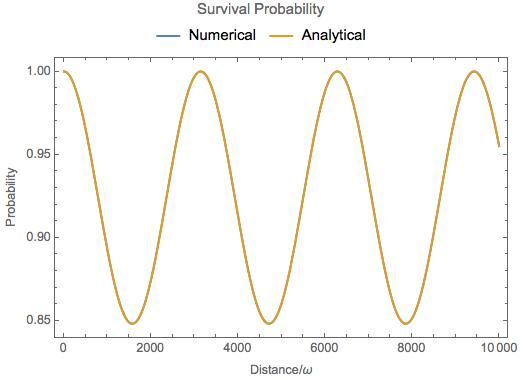
\includegraphics{assets/vacuumOsc}
\caption{They overlap on all the range completely.}
\end{marginfigure}




\subsection{Three Flavor States}

For three flavor neutrinos, the oscillations matrix is 3 by 3 which is called the PMNS matrix.

\begin{equation*}
\mathbf U = \begin{pmatrix}
U_{11} & U_{12} & U_{13} \\
U_{21} & U_{22} & U_{23} \\
U_{31} & U_{32} & U_{33}
\end{pmatrix},
\end{equation*}

which acts on the mass eigenstates to give the flavor eigenstates, i.e.,

\begin{equation*}
\ket{\nu_\alpha}= \mathbf{U}\ket{\nu_i}.
\end{equation*}

where

\begin{equation*}
\mathbf{U} = \begin{pmatrix}
U_{e1} & U_{e2} & U_{e3} \\
U_{\mu 1} & U_{\mu 2} & U_{\mu 3}\\
U_{\tau 1} & U_{\tau 2} & U_{\tau 3}
\end{pmatrix}.
\end{equation*}


In general, a rotation for 3D with a CP violation phase $\delta$ is

% A new command that scales down the size of the matrix
\newcommand\scalemath[2]{\scalebox{#1}{\mbox{\ensuremath{\displaystyle #2}}}}

\begin{equation*}
\mathbf{U} = \left(
\scalemath{0.8}{
\begin{array}{ccc}
 \cos \left(\theta _{12}\right) \cos \left(\theta _{13}\right) & \cos \left(\theta _{13}\right) \sin \left(\theta _{12}\right) & e^{-i \delta _{\text{CP}}} \sin \left(\theta _{13}\right) \\
 -\cos \left(\theta _{23}\right) \sin \left(\theta _{12}\right)-e^{i \delta _{\text{CP}}} \cos \left(\theta _{12}\right) \sin \left(\theta _{13}\right) \sin \left(\theta _{23}\right) & \cos \left(\theta _{12}\right) \cos \left(\theta _{23}\right)-e^{i \delta _{\text{CP}}} \sin \left(\theta _{12}\right) \sin \left(\theta _{13}\right) \sin \left(\theta _{23}\right) & \cos \left(\theta _{13}\right) \sin \left(\theta _{23}\right) \\
 \sin \left(\theta _{12}\right) \sin \left(\theta _{23}\right)-e^{i \delta _{\text{CP}}} \cos \left(\theta _{12}\right) \cos \left(\theta _{23}\right) \sin \left(\theta _{13}\right) & -e^{i \delta _{\text{CP}}} \cos \left(\theta _{23}\right) \sin \left(\theta _{12}\right) \sin \left(\theta _{13}\right)-\cos \left(\theta _{12}\right) \sin \left(\theta _{23}\right) & \cos \left(\theta _{13}\right) \cos \left(\theta _{23}\right) \\
\end{array}
}
\right).
\end{equation*}


However, with the CP violation phase $\delta$ this matrix is not unitary thus I'll choose $\delta=0$ for simplicity.\footnote{The effect of the phase can also be studied easily with the help of Mathematica.}

Now the matrix becomes,


\begin{equation*}
\mathbf{U} = \left(
\scalemath{0.8}{
\begin{array}{ccc}
 \cos \left(\theta _{12}\right) \cos \left(\theta _{13}\right) & \cos \left(\theta _{13}\right) \sin \left(\theta _{12}\right) & \sin \left(\theta _{13}\right) \\
 -\cos \left(\theta _{23}\right) \sin \left(\theta _{12}\right)-\cos \left(\theta _{12}\right) \sin \left(\theta _{13}\right) \sin \left(\theta _{23}\right) & \cos \left(\theta _{12}\right) \cos \left(\theta _{23}\right)-\sin \left(\theta _{12}\right) \sin \left(\theta _{13}\right) \sin \left(\theta _{23}\right) & \cos \left(\theta _{13}\right) \sin \left(\theta _{23}\right) \\
 \sin \left(\theta _{12}\right) \sin \left(\theta _{23}\right)-\cos \left(\theta _{12}\right) \cos \left(\theta _{23}\right) \sin \left(\theta _{13}\right) & -\cos \left(\theta _{23}\right) \sin \left(\theta _{12}\right) \sin \left(\theta _{13}\right)-\cos \left(\theta _{12}\right) \sin \left(\theta _{23}\right) & \cos \left(\theta _{13}\right) \cos \left(\theta _{23}\right) \\
\end{array}
}
\right).
\end{equation*}




The survival probability is given by the same derivation as the 2 flavor example. First of all we need to find the Hamiltonian in flavor basis from the propagation Hamiltonian, which is 

\begin{align*}
\mathbf{H} &= \mathbf{U} \mathbf{H_p} \mathbf{U^{-1}} \\
& = 
\left(
\scalemath{0.25}{
\begin{array}{ccc}
 \left(\cos ^2\left(\theta _{12}\right) m_1^2+\sin ^2\left(\theta _{12}\right) m_2^2\right) \cos ^2\left(\theta _{13}\right)+\sin ^2\left(\theta _{13}\right) m_3^2 & \frac{1}{2} \left(\cos \left(\theta _{13}\right) \cos \left(\theta _{23}\right) \sin \left(2 \theta _{12}\right) \left(m_2^2-m_1^2\right)+\sin \left(2 \theta _{13}\right) \sin \left(\theta _{23}\right) \left(-\cos ^2\left(\theta _{12}\right) m_1^2-\sin ^2\left(\theta _{12}\right) m_2^2+m_3^2\right)\right) & \frac{1}{2} \left(\cos \left(\theta _{13}\right) \sin \left(2 \theta _{12}\right) \sin \left(\theta _{23}\right) \left(m_1^2-m_2^2\right)+\cos \left(\theta _{23}\right) \sin \left(2 \theta _{13}\right) \left(-\cos ^2\left(\theta _{12}\right) m_1^2-\sin ^2\left(\theta _{12}\right) m_2^2+m_3^2\right)\right) \\
 \frac{1}{2} \left(\cos \left(\theta _{13}\right) \cos \left(\theta _{23}\right) \sin \left(2 \theta _{12}\right) \left(m_2^2-m_1^2\right)+\sin \left(2 \theta _{13}\right) \sin \left(\theta _{23}\right) \left(-\cos ^2\left(\theta _{12}\right) m_1^2-\sin ^2\left(\theta _{12}\right) m_2^2+m_3^2\right)\right) & \left(\cos \left(\theta _{23}\right) \sin \left(\theta _{12}\right)+\cos \left(\theta _{12}\right) \sin \left(\theta _{13}\right) \sin \left(\theta _{23}\right)\right){}^2 m_1^2+\left(\cos \left(\theta _{12}\right) \cos \left(\theta _{23}\right)-\sin \left(\theta _{12}\right) \sin \left(\theta _{13}\right) \sin \left(\theta _{23}\right)\right){}^2 m_2^2+\cos ^2\left(\theta _{13}\right) \sin ^2\left(\theta _{23}\right) m_3^2 & \frac{1}{8} \left(4 \cos \left(2 \theta _{23}\right) \sin \left(2 \theta _{12}\right) \sin \left(\theta _{13}\right) \left(m_1^2-m_2^2\right)-2 \cos \left(2 \theta _{13}\right) \sin \left(2 \theta _{23}\right) \left(\cos ^2\left(\theta _{12}\right) m_1^2+\sin ^2\left(\theta _{12}\right) m_2^2-m_3^2\right)+\sin \left(2 \theta _{23}\right) \left(\left(3 \cos \left(2 \theta _{12}\right)-1\right) m_1^2-\left(3 \cos \left(2 \theta _{12}\right)+1\right) m_2^2+2 m_3^2\right)\right) \\
 \frac{1}{2} \left(\cos \left(\theta _{13}\right) \sin \left(2 \theta _{12}\right) \sin \left(\theta _{23}\right) \left(m_1^2-m_2^2\right)+\cos \left(\theta _{23}\right) \sin \left(2 \theta _{13}\right) \left(-\cos ^2\left(\theta _{12}\right) m_1^2-\sin ^2\left(\theta _{12}\right) m_2^2+m_3^2\right)\right) & \frac{1}{8} \left(4 \cos \left(2 \theta _{23}\right) \sin \left(2 \theta _{12}\right) \sin \left(\theta _{13}\right) \left(m_1^2-m_2^2\right)-2 \cos \left(2 \theta _{13}\right) \sin \left(2 \theta _{23}\right) \left(\cos ^2\left(\theta _{12}\right) m_1^2+\sin ^2\left(\theta _{12}\right) m_2^2-m_3^2\right)+\sin \left(2 \theta _{23}\right) \left(\left(3 \cos \left(2 \theta _{12}\right)-1\right) m_1^2-\left(3 \cos \left(2 \theta _{12}\right)+1\right) m_2^2+2 m_3^2\right)\right) & \left(\cos \left(\theta _{12}\right) \cos \left(\theta _{23}\right) \sin \left(\theta _{13}\right)-\sin \left(\theta _{12}\right) \sin \left(\theta _{23}\right)\right){}^2 m_1^2+\left(\cos \left(\theta _{23}\right) \sin \left(\theta _{12}\right) \sin \left(\theta _{13}\right)+\cos \left(\theta _{12}\right) \sin \left(\theta _{23}\right)\right){}^2 m_2^2+\cos ^2\left(\theta _{13}\right) \cos ^2\left(\theta _{23}\right) m_3^2 \\
\end{array}
}
\right)
\end{align*}

where 
\begin{align*}
\mathbf{H_p} = \begin{pmatrix}
m_1^2 & 0 & 0 \\
0 & m_2^2 & 0 \\
0 & 0 & m_3^2
\end{pmatrix}.
\end{align*}

The next step is to define 

\begin{align*}
\Delta m_{12}^2 &= m_1^2 - m_2^2 \\
\Delta m_{23}^2 &= m_2^2 - m_3^2 
\end{align*}

so that they simplifies the Hermitian Hamiltonian to

\begin{equation*}
\mathbf{H} = 
\begin{pmatrix}
H_{11} & H_{12} & H_{13} \\
H_{21} & H_{22} & H_{23} \\
H_{31} & H_{32} & H_{33}
\end{pmatrix},
\end{equation*}

where \footnote{Haven't being copied from Mathematica code.}

\begin{align*}
H_{11} & = \cos^2\theta_{13}( m_2^2 - \sin^2\theta  \Delta m_{12}^2 ) + \sin^2\theta_{13} m_3^2 
\end{align*}




\begin{figure}
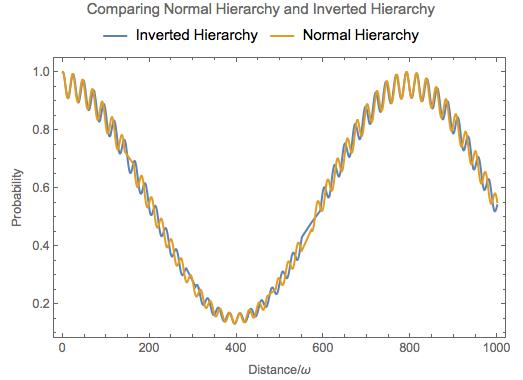
\includegraphics{assets/vacOsc3Flavor}
\caption{The overall shape is the same however they differ on small scales.}
\end{figure}


\begin{figure}
\centering
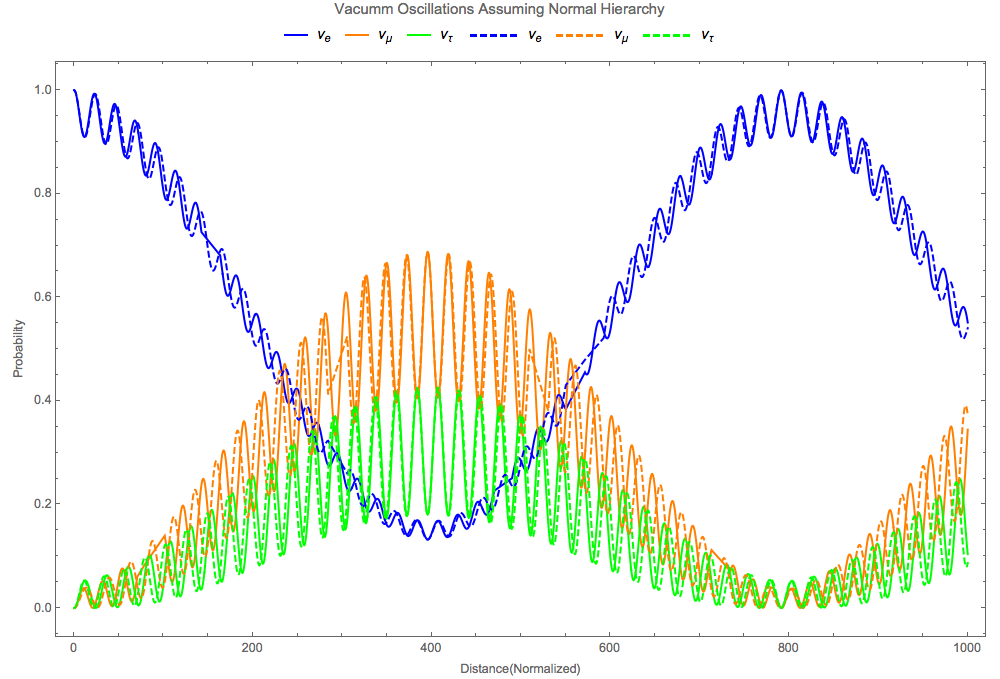
\includegraphics{assets/vacOscNormInvComp}
\caption{Comparison of normal hierarchy and inverted hierarchy.The reason that they are almost the same is that the oscillation length for $\Delta m_{13}^2$ is small thus it only changes the oscillation patterns for the small oscillations. Vacuum energy scales in normal hierarchy are
$$\omega_{12}= \frac{\Delta m_{12}^2}{2E} = 3.8\times 10^{-20}\mathrm{GeV}$$
$$\omega_{13}= \frac{\Delta m_{13}^2}{2E} = 1.7\times 10^{-18}\mathrm{GeV}$$
$$\omega_{23}= \frac{\Delta m_{23}^2}{2E} \approx \omega_{13}$$
 which shows that basically only two scales and the larger one determines the small oscillation.}
\label{fig:vacOscNormInvComp}
\end{figure}



\begin{figure}
\centering
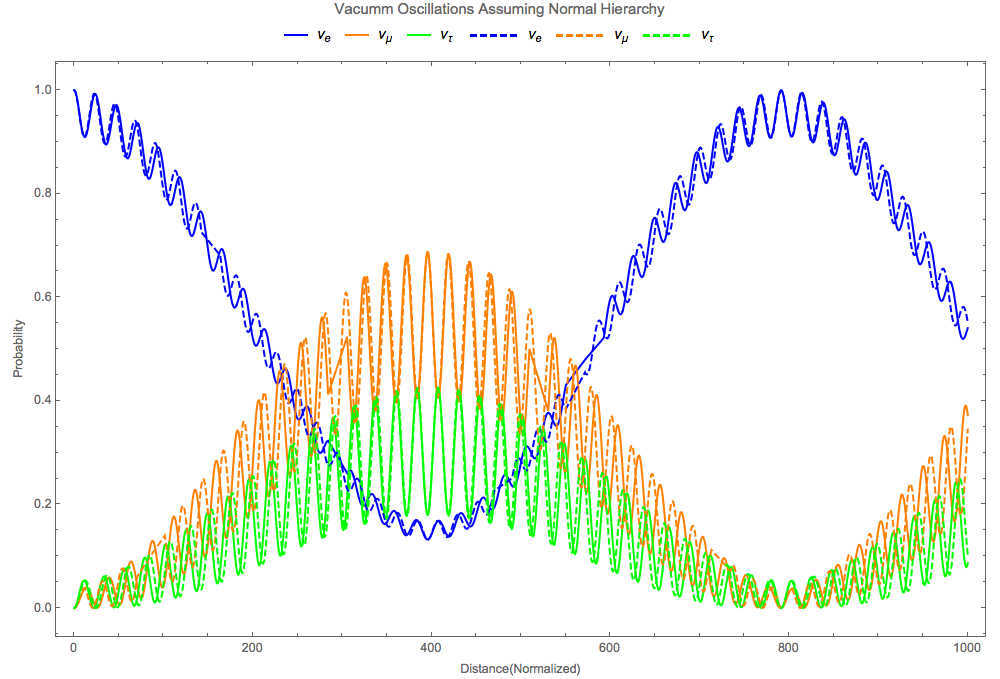
\includegraphics{assets/vacOscNormInvComp-Invert12.png}
\caption{Comparison of normal hierarchy and inverted hierarchy but with inverted $\Delta m_{12}^2$.}
\label{fig:vacOscNormInvComp-Invert12}
\end{figure}




\subsection{Ternary Diagram for Neutrino Flavor Oscillation}

Since the probability for differential flavors of neutrinos are represented in barycentric coordinates\footnote{They sum up to 1.}, a ternary plot would be nice to representation the oscillations. An example is shown in figure \ref{fig:ternaryPlot900}.





\begin{figure}
\centering
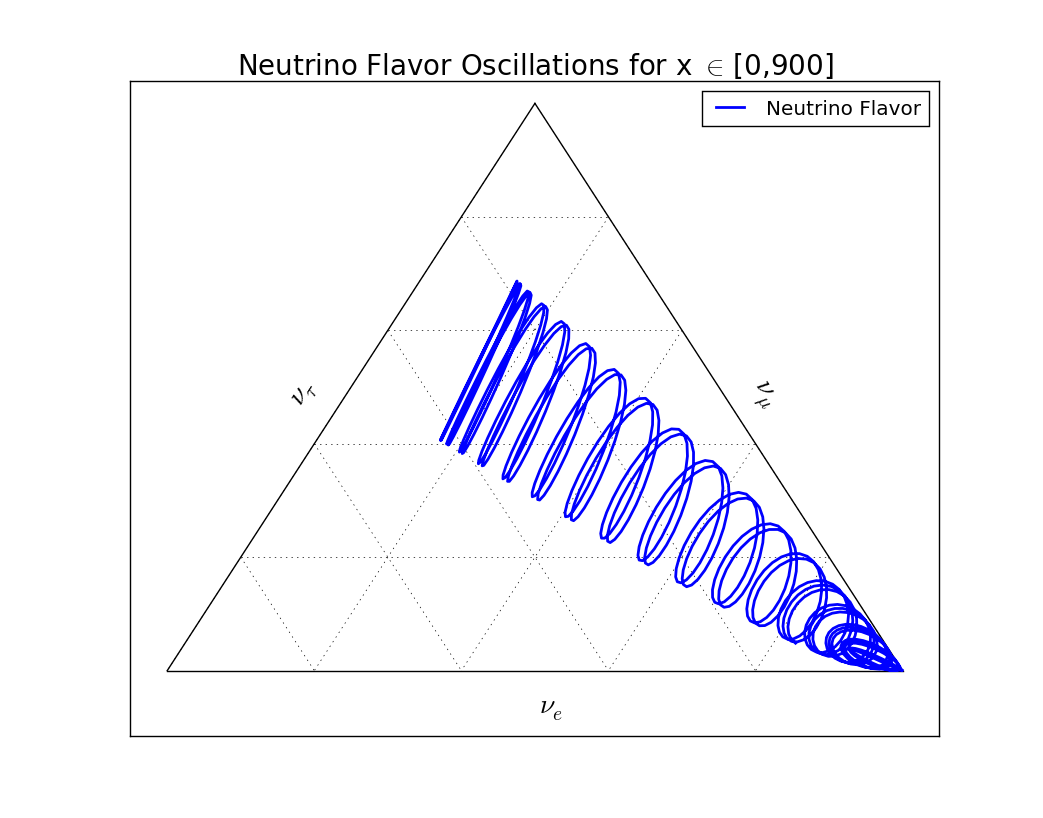
\includegraphics{assets/vacOsc3FlavorTernary900}
\caption{Ternary diagram for neutrino oscillations. The state starts from bottom left, which means that the system has only electron neutrinos. As the neutrino travels, it oscillates in curves. After one period of the beat, it reaches the far end and then oscillates backwards.}\
\label{fig:ternaryPlot900}
\end{figure}



\begin{marginfigure}
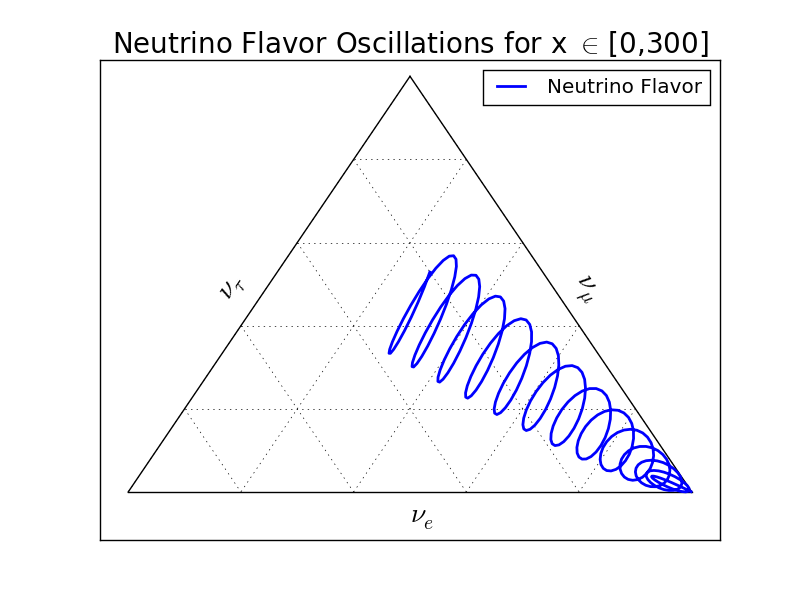
\includegraphics{assets/vacOsc3FlavorTernary300}
%\caption{This plot shows the behavior of neutrino oscillations in the range [0,300].}
\end{marginfigure}


\begin{marginfigure}
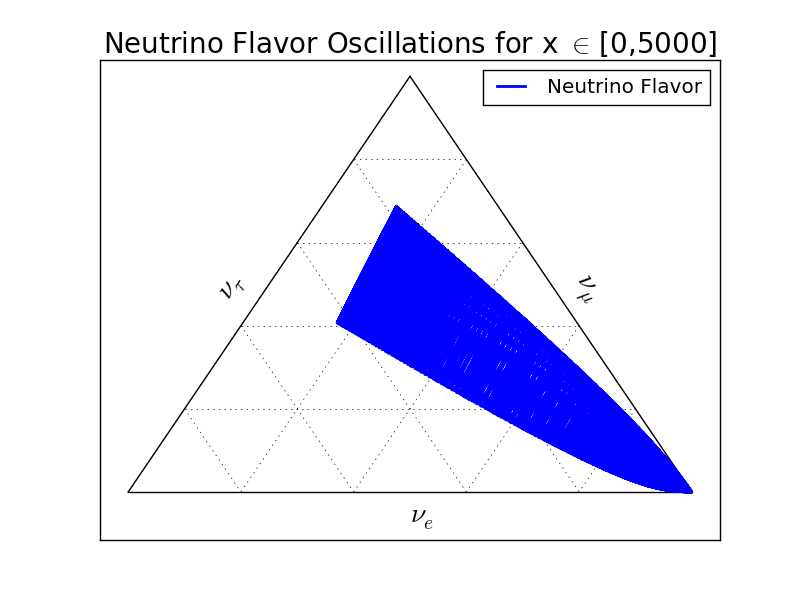
\includegraphics{assets/vacOsc3FlavorTernary5000}
%\caption{This plot shows the behavior of neutrino oscillations in the range [0,5000].}
\end{marginfigure}





\begin{figure}
\centering
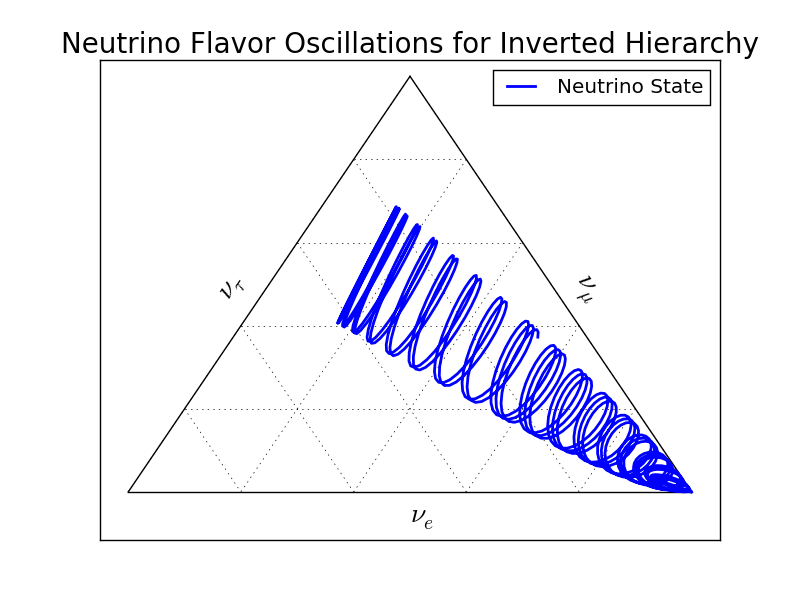
\includegraphics{assets/ternary/Inv-1000-1.png}
\caption{Ternary diagrram for inverted hierarchy.}
\label{fig:Inv-1000-1}
\end{figure}










%%%%%%%%%%%%%%%%%%%%%%%%%%%%%%%%%%%%
%%%%%  Oscillations in Matter
%%%%%%%%%%%%%%%%%%%%%%%%%%%%%%%%%%%%%

\section{Oscillations in Matter}


The Hamiltonian should be determined first. We have already derived the Hamiltonian for vacuum oscillation,

\begin{equation*}
H_v=\frac{ \delta m^2 }{2E}\frac{1}{2}\begin{pmatrix} -\cos 2\theta_v & \sin 2 \theta_v \\ \sin 2\theta_v & \cos 2\theta_v  \end{pmatrix},
\end{equation*}


where we would like to define a new matrix,

\begin{equation*}
\mathbf B = \frac{1}{2}\begin{pmatrix}  -\cos 2\theta_v & \sin 2 \theta_v \\ \sin 2\theta_v & \cos 2\theta_v  \end{pmatrix},
\end{equation*}


so that the vacuum Hamiltonian can be written as

\begin{equation*}
H_v = \frac{ \delta m^2 }{2E}\mathbf B.
\end{equation*}

The effect of matter, adds an extra term to this vacuum Hamiltonian which makes the electron population weighs more,

\begin{equation*}
H_m = \sqrt{2}G_F n_e L.
\end{equation*}

Here we have \footnote{In principle we could shift the Hamiltonian using an identity matrix $\alpha \mathbf{I}$ without change the eigenvectors. We will use an term $\frac{1}{2}\mathbf{\sigma_3} $ instead in the following sections.}

\begin{equation*}
L = \begin{pmatrix} 1 & 0 \\ 0 & 0 \end{pmatrix}.
\end{equation*}


Without emphasizing the self-interaction of the neutrinos, the Hamiltonian to be used is

\begin{equation}
H = H_v + H_m.
\end{equation}

The equation of motion is simply the von Neumann equation

\begin{equation}
i \partial_t \rho = \left[ H , \rho\right],
\end{equation}

in which the $\partial_t$ operator is actually $\partial_x$ since we always assume neutrinos travel with speed of light $c$.

A simple analysis before solving the system can be done rather easily. The characteristic length of the matter effect is

\begin{equation*}
l_m = \frac{2\pi}{\sqrt{2}G_F n} .
\end{equation*}

The importance of this length is that it is a result of refractive index which causes the velocity difference thus changes the relative phase between $\nu_e$ and $\nu_x$.\cite{wolfensteinprd1979}


With the definition of oscillation length in matter, a comparison between this length and the vacuum oscillation length can be made. Choose $\Delta m_{21}^2=10^{-4}\times 10^{-18}\mathrm{GeV^{2}}$\footnote{Fermi constant is $G_F=1.17\times 10^{-5}\mathrm{GeV^{-2}}$.}, we have

\begin{align*}
l_v &= 4\times 10^{19}\pi \left( \frac{E}{10^{-3}} \right) \mathrm{GeV^{-1}} \\
l_m &=  1.2\times 10^{19}\pi \left( \frac{10^{-14}}{n} \right) \mathrm{GeV^{-1}}
\end{align*}

The two lenght are equal if

\begin{equation*}
\left(\frac{10^{-14}}{n} \right) = 3.3 \left( \frac{E}{10^{-3}}\right)
\end{equation*}

More comparison can be found in figures \ref{fig:comparisonVacOscLengthMatterLength} and \ref{fig:lengthComparison}.

\begin{figure}
\centering
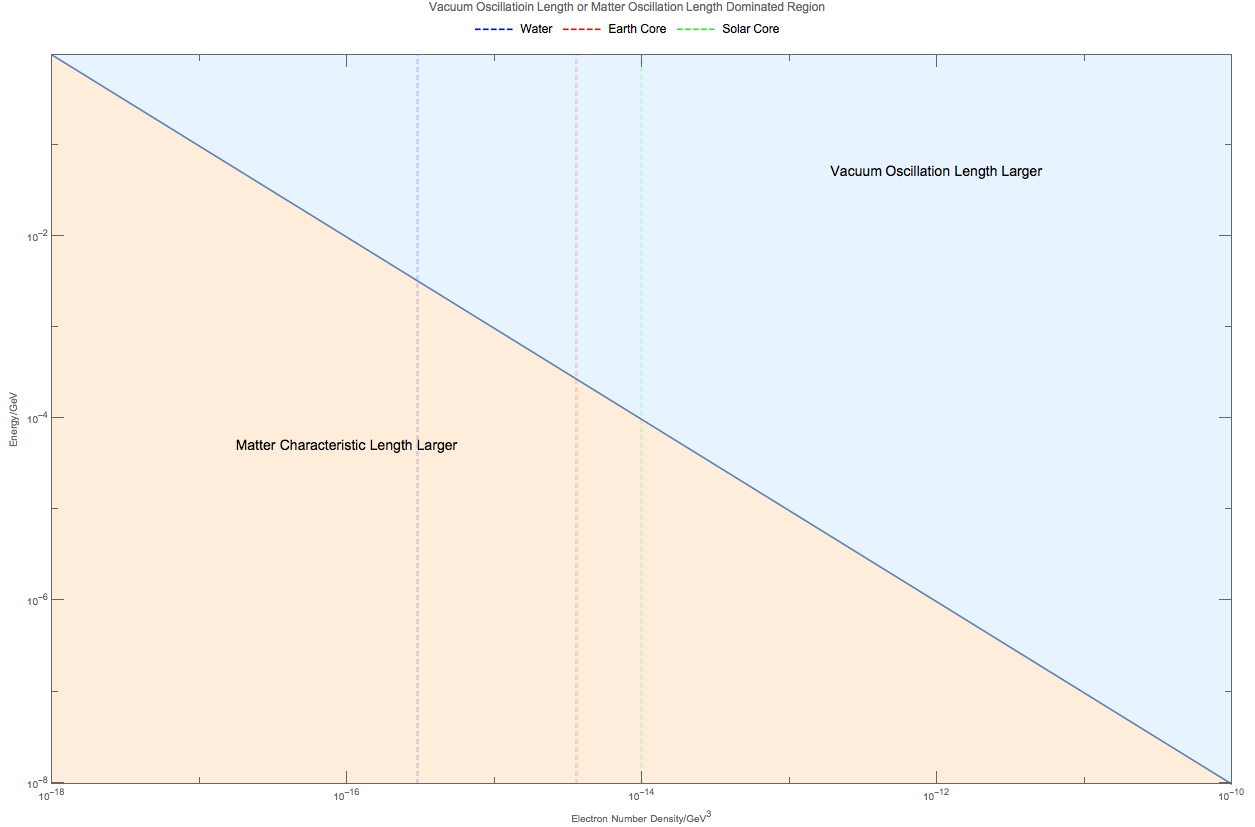
\includegraphics{assets/comparisonVacOscLengthMatterLength}
\caption{Comparison of the lengths}
\label{fig:comparisonVacOscLengthMatterLength}
\end{figure}


\begin{figure}
\centering
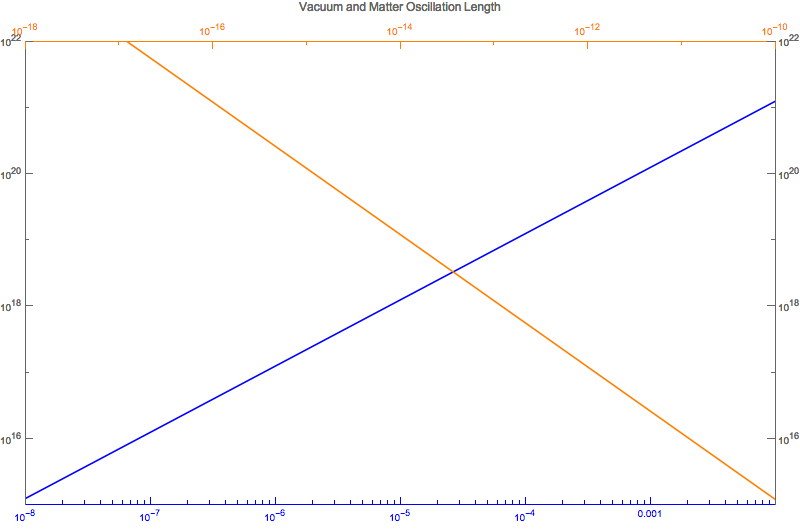
\includegraphics{assets/lengthComparison}
\caption{Comparison of the lengths}
\label{fig:lengthComparison}
\end{figure}







\subsection{Analytic Solution}


This Hamiltonian can be rewritten into a simple form using Pauli matrices,

\begin{align*}
\mathbf H &= \frac{ \Delta m^2 }{4E} \left( -\cos 2\theta_v \boldsymbol {\sigma}_3  + \sin 2\theta_v \boldsymbol{\sigma}_1 \right)  {\color{red} + \frac{\Delta}{2} \boldsymbol{\sigma}_3 } \\
& = \left(\frac{\Delta}{2} -\frac{ \Delta m^2 }{4E} \cos 2\theta_v \right) \boldsymbol{\sigma}_3  + \frac{ \Delta m^2 }{4E} \sin 2\theta_v \boldsymbol{\sigma}_1 \\
& = \left(\frac{\Delta}{2} -\frac{ \omega }{2} \cos 2\theta_v \right) \boldsymbol{\sigma}_3  + \frac{ \omega }{2} \sin 2\theta_v \boldsymbol{\sigma}_1,
\end{align*}

where $\Delta = \sqrt{2} G_F n(x) $ and $n(x)$ is the number density of the electrons.

To solve the equation of motion, this matrix should be diagonalized and its eigenvalues and eigenvectors should be identified. Since we have this Pauli matrices form, this can be done easily.

To see this effect quantitatively, we need to diagonalize this Hamiltonian (Can we actually diagonalize the equation of motion? NO!). Equivalently, we can rewrite it in the basis of mass eigenstates  $\{\ket{\nu_L(x)}, \ket{\nu_H(x)}\}$ \footnote{This is very different from the vacuum case since this one is local. In principle we can not use this transformation to diagonalize the Hamiltonian because the equation is a differential equation about $x$.} , 

\begin{align*}
\ket{\nu_L(x)} &= \cos\theta(x) \ket{\nu_e} - \sin\theta(x) \ket{\nu_\mu} \\
\ket{\nu_H(x)} & =  \sin\theta(x) \ket{\nu_e} + \cos\theta(x) \ket{\nu_\mu}.
\end{align*}


This new rotation in matrix form is 

\begin{marginfigure}
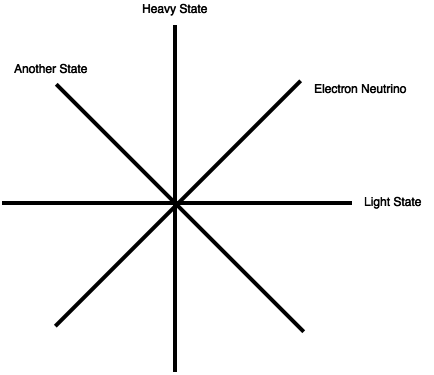
\includegraphics{assets/heavyLightRotation}
\caption{Due to this rotation, we can find an angle when the electron neutrinos becomes more important in Heavy state than Light state, which is $\theta=\frac{\pi}{4}$. For a mixing that has a larger angle, electron neutrinos actually take part in heavy neutrino state.}
\end{marginfigure}


\begin{align*}
\begin{pmatrix} \ket{\nu_L(x)} \\ \ket{\nu_H(x)} \end{pmatrix} &= \begin{pmatrix} \cos \theta(x) & -\sin\theta(x) \\ \sin\theta(x) & \cos\theta(x) \end{pmatrix} \begin{pmatrix}\ket{\nu_e} \\ \ket{\nu_x} \end{pmatrix} \\
& = \mathbf{U^{-1}_m } \begin{pmatrix}\ket{\nu_e} \\ \ket{\nu_x} \end{pmatrix} .
\end{align*}



To diagonalize it, we need to multiply on both sides the rotation matrix and its inverse, as we have done in the vacuum case,


\begin{equation*}
\mathbf {H_{md}} = \mathbf{U_m^{-1}} \mathbf H \mathbf {U_m}.
\end{equation*}

The second step is to set the off diagonal elements to zero. By solving the equations we can find the  $\sin 2\theta(x)$ and  $\cos 2\theta(x)$ . \footnote{Just remember that $\Delta = \sqrt{2}G_F n(x)$ is a function of position.}

\begin{align*}
\mathbf{H_{md}} &= \mathbf{U^{-1}_m} \left( A_1 \boldsymbol{ \sigma}_1  + A_3 \boldsymbol{\sigma}_3 \right) \mathbf{ U_m } \\
& = \begin{pmatrix} A_3\cos 2\theta(x) - A_1 \sin 2\theta(x) & A_3 \sin 2\theta(x) + A_1 \cos 2\theta(x) \\ A_3 \sin 2\theta(x) + A_1\cos 2\theta(x) &  - A_3 \cos 2\theta(x) + A_1 \sin 2\theta(x) \end{pmatrix},
\end{align*}

where

\begin{align*}
A_3 &  = \frac{\Delta}{2} - \frac{\delta^2 m}{4E}\cos 2\theta_v = \frac{\Delta}{2} - \frac{\omega}{2} \cos 2\theta_v \\
A_1 & =  \frac{\delta^2 m}{4E} \sin 2\theta_v = \frac{\omega}{2}\sin 2\theta_v.
\end{align*}

Set the off-diagonal elements to zero,

\begin{equation*}
A_3 \sin 2\theta(x) + A_1 \cos 2\theta(x)  = 0
\end{equation*}

So the solutions are

\begin{align*}
\sin 2\theta(x) & = \frac{A_1}{\sqrt{A_1^2 + A_3^2}}  \\
& = \frac{\sin 2\theta_v}{\sqrt{\hat\Delta^2 + 1 - 2\hat\Delta \cos 2\theta_v}}\\
\cos 2\theta(x) & = \frac{-A_3}{\sqrt{A_1^2+A_3^2}} \\
& = \frac{- (\hat\Delta - \cos 2\theta_v )}{ \sqrt{\hat\Delta^2 + 1 - 2\hat\Delta \cos 2\theta_v} } ,
\end{align*}

where $\hat\Delta = \Delta/\omega$.




This diagonalizes the Hamiltonian LOCALLY. \footnote{The point is, for equation of motion, we have a differentiation with respect to position  $x$ ! So even we diagonalize the Hamiltonian, the equation of motion won't be diagonalized. An extra matrix will occur on the LHS and revert the diagonalization the Hamiltonian on RHS.
} It's not possible to diagonalize the Hamiltonian globally if the electron number density is not a constant.

{\color{red}As for a qualitative analysis, matter effect can be a suppression or enhancement. $\sin 2\theta_v$ represents the amplitude of the survivable probability of one of the flavors since larger $\theta_v$ means more mixing between the two flavors. However matter changes the mixing angle according to the expression of $\sin 2\theta_m$, which is

\begin{itemize}
\item larger than $\sin 2\theta_v$ if $ 0 < \hat\Delta < 2\cos 2\theta_v$.
\item smaller than $\sin 2\theta_v$ if $\hat\Delta > 2\cos 2\theta_v$.
\end{itemize}

A smaller $\sin2\theta$ means a smaller mixing. Matter can sometimes suppress the mixing while can also enhance the mixing.}



As  $\Delta \to \infty$ ,  we have $A_3\to \infty$ and  $\sin 2\theta(x)$ vanishes. The effective mixing angle $\theta_m$ becomes $\pi/2$ thus only a phase is added to first mass eigenstate, i.e., $\ket{\nu_e}=-\ket{\nu_1}$ and $\ket{\nu_x}=\ket{\nu_2}$. Thus the neutrino will stay on the defined light and heavy eigenstates if the interaction with matter is much larger than the vacuum energy. On the other hand, $\Delta \to 0$, everything gets back to the vacuum case.

Now we can obtain an approximate solution by using this approximate diagonalization. This idea is

\begin{equation*}
i \partial_x \Psi_m(x) = \mathbf{Extra Matrix From LHS}\cdot \mathbf H_{md} \Psi_m(x),
\end{equation*}

where the $\mathbf{Extra Matrix From LHS}$ comes from the fact that changing from flavor basis $\Psi(x)$ to heavy-light basis $\Psi_m(x)$ using $\mathbf {U_m}$

\begin{equation*}
i\partial_x (\mathbf{U_m} \Psi_m(x)) = H ( \mathbf{U_m} \Psi_m(x) )
\end{equation*}

only returns

\begin{equation*}
i\partial_x \Psi_m(x) = \mathbf{H_{md} } \Psi_m(x) - i \mathbf{U_m^{-1}} ( \partial_x \mathbf{U_m} ) \Psi_m(x).
\end{equation*}

Combining the two terms on RHS,

\begin{equation*}
i\partial_x \Psi_m(x) = \mathbf{H_m} \Psi_m(x),
\end{equation*}

where

\begin{equation*}
\mathbf{H_m} = \mathbf{H_{md}} - i \mathbf{U_m^{-1}} ( \partial_x \mathbf{U_m} ).
\end{equation*}

The only part inside $\mathbf{U_m(x)}$ that is space dependent is the number density of the electrons $n(x)$. {\bf{Thus we know immediately that the Hamiltonian is diagonalized if the number density is constant.}}\footnote{But even the electrons density is constant, the oscillation is different.}\footnote{\bf It would be nice to find the expression of $\mathbf{U_m}$ in order to play with the matter effect.}\footnote{In a two level system, suppose the Hamiltonian is

\begin{equation*}
H_2 = H_{d2} + P_{2},
\end{equation*}

where 

\begin{align*}
H_{d2} & = \begin{pmatrix}
E_1 & 0 \\
0 & E_2
\end{pmatrix} \\
P_{2} & = \begin{pmatrix}
0 & W(r) \\
W^*(r) & 0 
\end{pmatrix}
\end{align*}

are the diagonalized Hamiltonian and the perturbation.

The diagonalized Hamiltonian will result in a system with two levels which are constant as a function of $r$, however the perturbation term provides the $r$ dependent term which will cause a $r$ dependent eigen energies.
}



{\color{red}In fact there are at least three different ways of solving this problem.
\begin{itemize}
\item Work in instantaneous eigenstates by writing down the general expression as we have done in this subsection.
\item Work in flavor basis directly.
\item Work in the vacuum mass eigenstates by transform the matter potential from flavor basis to vacuum mass basis.
\end{itemize}}


\subsection{Constant Electron Number Density}

Suppose we have an environment with constant electron number density, the term $- i \mathbf{U_m^{-1}} ( \partial_x \mathbf{U_m} )$ goes away. All we have is the diagonalized new Hamiltonian $\mathbf{H_{md}}$ and the eigenvalues are easily obtained which are

\begin{align*}
 E_1 &= A_3\cos 2\theta(x) - A_1 \sin 2\theta(x) \\ 
 E_2 & = - A_3 \cos 2\theta(x) + A_1 \sin 2\theta(x) .
\end{align*}

The final result for these two eigenvalues are

\begin{align*}
E_1 &= -\sqrt{A_1^2 + A_3^2} \\
E_2 &= \sqrt{A_1^2 + A_3^2},
\end{align*}

where

\begin{equation*}
A_1^2 + A_3^2 = \frac{\Delta^2 + \omega^2 }{4} - \frac{\Delta \omega }{2} \cos 2\theta_v.
\end{equation*}


There are two special cases. The first case is $\cos 2\theta_v=0$ while the other one is $\cos 2\theta_v = 1$ which leads to $\sqrt{A_1^2+A_3^2} = \lvert\frac{\Delta - \omega}{2} \rvert$ and the two energies becomes $\frac{\Delta - \omega}{2}$ and $\frac{\omega - \Delta}{2} $.\footnote{This means the matter effect in this constant profile situation determines the difference between the eigen energies.}


As for the survival probability, the result has the same form as the vacuum case, which is

\begin{equation*}
P_x(\nu_e,L) = 1 - \sin^2(2\theta_m)\sin^2\left( \frac{\omega_m L}{2} \right) ,
\end{equation*}



where $\theta_m = \theta(x)$ is the effective mixing angle which in fact doesn't depend on $x$ if the matter profile is constant.\footnote{The term $\sin 2\theta_m$ has been derived previously.
\begin{equation*}
\sin 2\theta(x)  = \frac{\omega\sin 2\theta_v}{\sqrt{ \omega^2+\Delta^2 - 2 \omega \Delta\cos 2\theta_v }}.
\end{equation*}
}

As an comparison, the vacuum result is

\begin{equation*}
P_x(\nu_e,L) = 1 - \sin^2(2\theta)\sin^2\left( \frac{\omega L}{2} \right) .
\end{equation*}

As the math tells us, $\sin^2 2\theta$ and $\sin^2 2\theta_m$ are the two terms that determines how much electron flavor is converted to the other flavor. The other parts determine the oscillation period.

Recall that we have defined two characteristic lengths, $l_v$ and $l_m$. The overall oscillation length in matter becomes\footnote{We know that $\omega>0$ here since we have already determined the hierarchy for $m_1$ and $m_2$. How? There is a significant effect on the oscillations here if $\omega<0$!}

\begin{align*}
l &= \frac{2\pi}{\omega_m} \\
& = \frac{2\pi}{\omega \sqrt{ \hat\Delta^2 + 1 - 2 \hat\Delta \cos 2\theta_v }} \\
& = \frac{l_v}{ \sqrt{\left(\frac{l_v}{l_m} \right)^2 +1 - 2\frac{l_v}{l_m}\cos 2\theta_v  }}
\end{align*}

This expression shows exactly why the different length scales are important.

\begin{itemize}
\item  $\lvert \frac{l_v}{l_m} \rvert \ll 1 \Rightarrow l\to l_v$, matter effect is minimal.
\item  $\lvert \frac{l_v}{l_m} \rvert \gg 1 \Rightarrow l\to 0 $, matter effect kills the oscillations.
\item  $\lvert \frac{l_v}{l_m}\rvert \sim 1 \Rightarrow l\to \frac{l_v}{2\sin\theta_v}$, more interesting region.\footnote{Assume $\sin\theta_v>0$.} To linear approximation, \begin{equation*}
l \approx \frac{l_v}{2\sin\theta_v} \left( 1 -  \frac{l_v/l_m - 1}{2} \right).
\end{equation*} notice that at resonance \begin{equation*}
l = \frac{l_v}{2\sin \theta_v}.
\end{equation*}
\end{itemize}


Another important thing about these lengths is that $l_v$ is a function of energy which is that higher energy means longer oscillation length as shown in figure \ref{fig:comparisonVacOscLengthMatterLength} and \ref{fig:lengthComparison}. This is important because we can always find the a energy that is at resonance with the matter density, as long as the energy still makes sure the neutrinos are relativistic. So a spectral swap is possible.



\subsection{Adiabatic Limit}



In some astrophysical environments the electron number density changes very slowly which means the term $\mathbf{U_m^{-1}} \partial_x \mathbf{U_m} $ is much smaller than $\mathbf{H_{md}}$. By intuition we would expect that this term could be dropped to the lowest order. However to verify that we need to check the Taylor expansion of this gradient term which requires the general form of $\mathbf{U_m}$.


Before we actually do the expansion, make the quantities dimensionless would greatly help us.

\begin{align*}
\sin 2\theta(x)  &= \frac{\sin 2\theta_v}{\sqrt{ \left(\frac{\Delta}{\omega} \right)^2+1 - 2 \frac{\Delta}{\omega}\cos 2\theta_v }} \\
\cos 2\theta(x)&= \frac{ \cos 2\theta_v - \frac{\Delta}{\omega} }{ \sqrt{ \left( \frac{\Delta}{\omega} \right)^2  +1 - 2 \frac{\Delta}{\omega}\cos 2\theta_v  }}.
\end{align*}

Define $\hat\Delta = \frac{\Delta}{\omega}$, which represents the matter interaction strength compared to the vacuum oscillation.

\begin{align*}
\sin 2\theta(x)  &= \frac{\sin 2\theta_v}{\sqrt{ \hat\Delta ^2+1 - 2 \hat\Delta \cos 2\theta_v }} \\
\cos 2\theta(x)&= \frac{ \cos 2\theta_v - \hat\Delta  }{ \sqrt{\hat\Delta ^2  +1 - 2 \hat\Delta \cos 2\theta_v } }.
\end{align*}



\begin{align*}
\sin\theta(x) & = \frac{\csc \left(2 \theta _v\right) \sqrt{\frac{-\hat{\Delta }+\sqrt{\hat{\Delta }^2-2 \hat{\Delta } \cos \left(2 \theta _v\right)+1}+\cos \left(2 \theta _v\right)}{\sqrt{\hat{\Delta }^2-2 \hat{\Delta } \cos \left(2 \theta _v\right)+1}}} \left(\hat{\Delta }+\sqrt{\hat{\Delta }^2-2 \hat{\Delta } \cos \left(2 \theta _v\right)+1}-\cos \left(2 \theta _v\right)\right)}{\sqrt{2}} \\
\cos\theta(x)& = \frac{\sqrt{\frac{-\hat{\Delta }+\sqrt{\hat{\Delta }^2-2 \hat{\Delta } \cos \left(2 \theta _v\right)+1}+\cos \left(2 \theta _v\right)}{\sqrt{\hat{\Delta }^2-2 \hat{\Delta } \cos \left(2 \theta _v\right)+1}}}}{\sqrt{2}}
\end{align*}


This is extremely complicated if we take the derivative with respect to $x$. So we apply Taylor expansion.\footnote{The $i$s are there makes sure that $-i\partial_x \mathbf{U_m}(x)$ is real.}

\begin{align*}
\frac{d \sin \theta(x)}{dx} &= \frac{d\sin \theta(x)}{d\hat\Delta}\frac{d\hat\Delta}{dx} \\
& = i \frac{d\hat\Delta}{dx} \left(  -cos\theta_v\sin^2\theta_v -\frac{1}{2} ( (1+5\cos 2\theta_v) \cos\theta_v \sin^2\theta_v ) \hat\Delta + \mathcal{O}(\hat\Delta^2) \right) \\
\frac{d\cos\theta(x)}{dx} & = \frac{d\cos\theta(x)}{d\hat\Delta}\frac{d\hat\Delta}{dx} \\
& = i \frac{d\hat\Delta}{dx}\left( cos^2\theta_v\sin\theta_v + \frac{1}{2}\cos^2\theta_v(-1+5\cos 2\theta_v) \sin\theta_v \hat\Delta + \mathcal{O}(\hat\Delta^2) \right)
\end{align*}

There is nothing in the coefficients that prohibits us from using the lowest order that $\frac{d\hat\Delta /dx}{\text{Energy Differences Between Two Energy Levels}}\ll 1$ since the Taylor series has finite values.\footnote{No singularities possible. I assumed that $\sin \theta_v >0$. }

Solving the adiabatic limit is just the same as the constant limit but $\theta(x)$ is not constant which ensures changing energies. What would be interesting is the behavior of energies as the density profile is slowing changing.

\begin{align*}
E_1 & = -\frac{\omega}{2}\sqrt{\hat\Delta^2 + 1 - 2 \hat\Delta  \cos 2\theta_v} \\
E_2 & = \frac{\omega}{2}\sqrt{\hat\Delta^2 + 1 - 2 \hat\Delta  \cos 2\theta_v}.
\end{align*}

When the term $\hat\Delta$ is very small $1-2\hat\Delta\cos 2\theta_v$ will dominate and the whole term decreases. On the other hand as $\hat\Delta$ becomes large, $\hat\Delta^2$ will dominate and the whole term grows.


\begin{marginfigure}
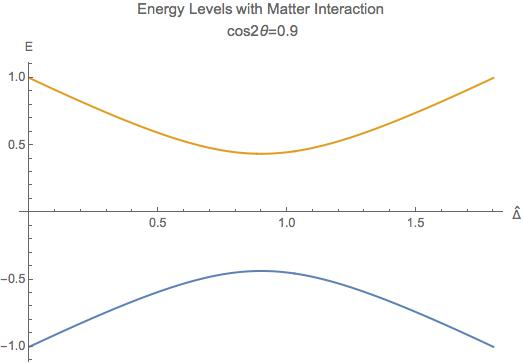
\includegraphics{assets/mswEnergyLevels}
\caption{Energy Levels for MSW effect. We have the up-down symmetry since we shifted the energy by a constant to remove the identity matrix in the Hamiltonian.}
\end{marginfigure}


The survival probability for the light neutrinos would be

\begin{equation*}
P_x(\nu_L,L) = 1 - \sin^2(2\theta (x))\sin^2\left( \frac{\omega L}{2} \right) .
\end{equation*}


The survival probability for electron flavor neutrino is

\begin{equation*}
P_x(\nu_e,L) = \frac{1}{2} + \frac{1}{2}\cos 2\theta(x_0) \cos 2\theta_v,
\end{equation*}

if the neutrinos are produced in dense region and the detection happens in vacuum.


Before we move on to higher order corrections, it would be nice to understand this phenomenon.


\begin{itemize}
\item
The vacuum oscillation length can be extracted from vacuum oscillation survival probability. It is $L_v = \frac{2\pi}{\omega}$.
\item
In this problem we have another energy scale which is the interaction, $\Delta$. Here we can define another characteristic length $l_m = \frac{2\pi}{\Delta}$.
\item 
MSW resonance happens when the two character lengths are matching to each other. Another way to put it is that the the term $\sin 2\theta(x)$ is minimized so that we have the smallest gap which leads to math $\hat\Delta = \cos 2\theta_v$. Equivalently this is the relation
\begin{equation*}
l_0 = l_m\cos 2\theta_v.
\end{equation*}
\item
At resonance, we have
\begin{align*}
\cos 2\theta(x) &= 1 \\
\sin 2\theta(x) &= 0.
\end{align*}

This is max mixing of the states which means that at the resonance point

\begin{equation*}
\begin{pmatrix} \nu_L(x_{reso}) \\ \nu_H(x_{reso}) \end{pmatrix} = \frac{\sqrt{2}}{2}\begin{pmatrix} 1 & -1 \\ 1 & 1 \end{pmatrix} \begin{pmatrix}\nu_e \\ \nu_x \end{pmatrix}
\end{equation*}

\item

Resonance conditions corresponds to a resonance density which is given by

\begin{equation*}
n_e(x) = \frac{\omega}{\sqrt{2}G_F } \cos 2\theta_v \equiv n_0(E,\Delta m^2) \cos 2\theta_v,
\end{equation*}

where $n_0(E,\Delta m^2)$ is a characteristic number density which depends on the energy mixing angles and $\Delta m^2$ of the neutrinos.


\item
One should notice that to get back to the vacuum oscillation survival probability which means $\sin^2 2\theta(x) = \sin^2 2\theta_v $ we have\footnote{\bf I should check if this is still true in 3 flavor neutrino scenario. This could be interesting if it is respected in 3 flavor neutrino oscillations.}

\begin{equation*}
\hat\Delta^2 + 1 - 2\hat\Delta \cos 2\theta_v = 1,
\end{equation*}

which leads to

\begin{equation*}
\hat\Delta = 0 \quad\text{or}\quad 2\cos 2\theta_v .
\end{equation*}

The first condition is trivial which corresponds to vacuum however the second condition $\Delta = 2\cos 2\theta_v \omega$ means the interaction oscillation length is doubled compared to resonance point.

{\bf{Nevertheless, we should always remember to check what survival probability the expression is describing. Here we have survival probability for $\nu_L(x)$. At $n(x)\to 0$ the oscillation becomes vacuum oscillation.}}

\end{itemize}




\subsection{First Order Approximation}


In principle we could use Taylor expansion of $\mathbf{U_m}$ to find the series of the derivatives of $\cos\theta(x)$ and $\sin\theta(x)$, however it doesn't looks like the easy way. Now we go back to find the Taylor expansion of the Hamiltonian which only involves the expression $\sin 2\theta(x)$ and $\cos 2\theta(x)$.

The series of them are

\begin{align*}
\sin 2\theta(x) & = \sin 2\theta_v + \cos 2\theta_v \sin 2\theta_v \hat\Delta + \mathcal{O}(\hat\Delta)^2 \\
\cos 2\theta(x) & = \cos 2\theta_v -\sin^2 2\theta_v \hat \Delta + \mathcal{O}(\hat\Delta)^2 .
\end{align*}

Notice that for small $\theta_v$ the first order can be neglected sine they are second or higher order small quantities.

$\sin\theta(x)$ and $\cos\theta(x)$ can be found using these results.

\begin{align*}
\sin\theta(x) & = \sin \theta_v + \cos^2\theta_v \sin\theta_v \hat\Delta + \mathcal{O}(\hat\Delta^2) \\
\cos\theta(x) & = \cos\theta_v - \cos\theta_v \sin^2\theta_v \hat\Delta + \mathcal{O}(\hat\Delta^2).
\end{align*}

To find out the solutions the explicit expression for $\mathbf{U_m}$ is required. The rotation matrix is

\begin{align*}
\mathbf{U_m} &= \begin{pmatrix} \cos \theta(x) & \sin\theta(x) \\ -\sin\theta(x) & \cos\theta(x) \end{pmatrix} \\
&\approx \begin{pmatrix}
\cos\theta_v - \cos\theta_v \sin^2\theta_v \hat\Delta &  \sin \theta_v + \cos^2\theta_v \sin\theta_v \hat\Delta \\
-  \sin \theta_v - \cos^2\theta_v \sin\theta_v \hat\Delta & \cos\theta_v - \cos\theta_v \sin^2\theta_v \hat\Delta
\end{pmatrix}.
\end{align*}

The derivative of this rotation matrix with respect to $x$ is

\begin{align*}
\partial_x \mathbf{U_m} & = \frac{d \hat\Delta}{dx} \begin{pmatrix}
 - \cos\theta_v \sin^2\theta_v  &  \cos^2\theta_v \sin\theta_v  \\
 - \cos^2\theta_v \sin\theta_v  &  - \cos\theta_v \sin^2\theta_v 
\end{pmatrix}
\end{align*}


The effective potential is\footnote{This expression comes from the result of the first order approximation of $\sin\theta(x)$ and $\cos\theta(x)$.}

\begin{align*}
\mathbf{V_m} & = -i\mathbf{U_m^{-1}} ( \partial_x \mathbf{U_m} ) \\
& = - i\sin\theta_v \cos\theta_v \frac{d\hat\Delta}{dx} \begin{pmatrix}
\cos\theta_v\sin\theta_v \hat \Delta & 1 \\
-1 & \cos\theta_v \sin\theta_v \hat\Delta 
\end{pmatrix} .
\end{align*}

Since $\frac{d\hat\Delta}{dx} \hat\Delta$ is one order higher than $\hat\Delta$, the effective potential can be simplified to first order, which is

\begin{align*}
\mathbf{V_m} & = - i\sin\theta_v \cos\theta_v \frac{d\hat\Delta}{dx} \begin{pmatrix}
0 & 1 \\
-1 & 0
\end{pmatrix}.
\end{align*}

The equation of motion up to first order of $\hat\Delta$ becomes

\begin{equation*}
i\partial_x\ket{\Psi_m} = (\mathbf{H_{md}} + \mathbf{V_m})\ket{\Psi_m}.
\end{equation*}

We have already solved
\begin{equation*}
i\partial_x\ket{\Psi_m} = \mathbf{H_{md}} \ket{\Psi_m},
\end{equation*}

where the eigenstates are $\ket{\nu_L}$ and $\ket{\nu_H}$.


In general we define

\begin{equation*}
v = -\sin\theta_v \cos\theta_v\frac{d\hat\Delta}{dx}
\end{equation*}

so that

\begin{equation*}
\mathbf{V_m} = \begin{pmatrix}
0 & i v \\
-i v & 0
\end{pmatrix}.
\end{equation*}

The general solution to the equation we need to solve can be written as

\begin{equation*}
\ket{\Psi_m} = C_L(x) e^{-i\int \omega_{m1} dx} \ket{\nu_L} + C_H(x) e^{-i\int \omega_{m2} dx} \ket{\nu_H},
\end{equation*}

where

\begin{align*}
\omega_{m1} &=-\sqrt{ \frac{\Delta^2 + \omega^2}{4}-\frac{\Delta \omega}{2} \cos 2\theta_v } \\
& = -\omega \sqrt{\left( \frac{\hat\Delta^2 + 1}{4} - \frac{\hat\Delta}{2}\cos 2\theta_v \right)} , \\
\omega_{m2} & = - \omega_{m1} \equiv \frac{\omega_m}{2}.
\end{align*}

Hamiltonian applied to this state results in

\begin{align*}
\mathbf{H_m} \ket{\Psi_m} =& \omega_{m1} C_L(x) e^{-i\int \omega_{m1}dx} \ket{\nu_L} -ivC_L(x) e^{-i\int \omega_{m1}dx}\ket{\nu_H} \\ &+\omega_{m2}C_H(x) e^{-i\int \omega_{m2}dx}\ket{\nu_H} + iv C_H(x) e^{-i\int \omega_{m2}dx}\ket{\nu_L}.
\end{align*}

Plug the state $\ket{\Psi_m}$ into the Schrödinger equation, we have

\begin{align*}
\dot C_L(x) &= v C_H(x) e^{ - i\int \delta \omega_m dx} \\
\dot C_H(x) & = -v C_L(x) e^{i\int \delta\omega_m dx} ,
\end{align*}

in which $\delta\omega_m$ is defined as

\begin{equation*}
\delta \omega_m = \omega_{m2} - \omega_{m1}.
\end{equation*}


The first order differential equations of $C_L(x)$ and $C_H(x)$ can be combined and produce a second order differential equation.

\begin{equation*}
\ddot C_L - \left(  \frac{\dot v}{v} - i\delta \omega_m \right) \dot C_L + v^2 C_L = 0.
\end{equation*}

In our linear approximation that $\frac{d\hat\Delta}{dx}$ is a constant.\footnote{We are assuming that $n(x)$ is linearly depending on $x$ which means $\hat\Delta$ is a linear function of $x$. Thus $\frac{d\hat\Delta}{dx}$ is a constant.} The equation simplifies to

\begin{equation*}
\ddot C_L + i\delta\omega_m \dot C_L + v^2 C_L = 0,
\end{equation*}

where $v=-\sin\theta_v\cos\theta_v \frac{d\hat\Delta}{dx}$ is constant.

Assuming one of the solutions is $e^{rx}$, we could insert it to the second order differential equation and get the characteristic equation,

\begin{equation*}
r^2 + i\delta \omega_m r + v^2 = 0,
\end{equation*}

which has two solutions

\begin{align*}
r_1 & =  i \frac{-\delta\omega_m + \sqrt{\delta\omega_m+ 4v^2} }{2} \\
r_2 & = i\frac{-\delta\omega_m - \sqrt{\delta\omega_m+ 4v^2} }{2}.
\end{align*}

The solutions to $C_L(x)$ and $C_H(x)$ will be

\begin{align*}
C_L(x) & = c_1 e^{r_1 x} + c_2 e^{r_2 x} \\
C_H(x) & = \left( c_1 e^{r_1 x} + c_2 e^{r_2 x} \right) \frac{ e^{ i\int \delta\omega_m dx } }{v} .
\end{align*}

These constants are determined by the initial condition. The state of the system at any $x$ is

\begin{align*}
\ket{\Psi_m(x)} = & \left( c_1 e^{r_1 x} + c_2 e^{r_2 x} \right) e^{-i\int_0^x \omega_{m1}(x') dx'} \ket{\nu_L}  \\
& + \left( c_1 e^{r_1 x} + c_2 e^{r_2 x} \right) \frac{ e^{ i\int \delta\omega_m dx } }{v} e^{-i\int_0^x \omega_{m2}(x') dx'} \ket{\nu_H}.
\end{align*}


Suppose we have the initial condition as $\ket{\Psi_m(x=0)} = \ket{\nu_L}$, the system can jump to $\ket{\nu_H}$ since the state at arbitrary position $x$ is a mixing of the two states.\footnote{In fact this approximation is valid at the level crossing.} The rate of jumping is given by\cite{Vutha2010,Zener1932,Rubbmark1981}

\begin{equation*}
\Gamma = \frac{(2v )^2}{4\left( \frac{d\omega_m}{dx} \right)} = \frac{v^2}{\frac{d\omega_m}{dx}}.
\end{equation*}


The probability jumping to state $\ket{\nu_H}$ after the level crossing (at infinite $x$) is

\begin{align*}
P(x\to \infty, \ket{\nu_L}\to\ket{\nu_H}) &= e^{-2\pi\Gamma} \\
& = \exp\left( -2\pi \frac{v^2}{\frac{d\omega_m}{dx}} \right) \\
& = \exp\left( -2\pi \frac{\left( -\sin\theta_v\cos\theta_v \frac{d\hat\Delta}{dx}  \right)^2}{\frac{d\omega_m}{dx}} \right).
\end{align*}

The survival probability can be calculated by counting the probability left on the initial state.

To be clear, if electron neutrinos are produced inside core of our sun, it will be the light state. Since the interaction with matter is very strong, it transfers to $\ket{\nu_L}$ with probability $P(x\to \infty, \ket{\nu_L}\to\ket{\nu_H}) $ due to the gradient of the matter profile which works as the perturbation. Thus the final state will be a mixing of $\ket{\nu_L}$ and $\ket{\nu_H}$.






\subsection{General Discussion for Neutrinos Interacting with Matter}


This part is a very general discussion of the matter effect.\cite{Parke1986}

To work in flavor basis, we use the subscript ${}_{mf}$ to denote the flavor basis representation with mass effect. The equation of motion in flavor basis can be written down as\footnote{Writing down the dimensionless equation, I have 
\begin{equation*}
i \partial_{\hat x} \Psi_{mf} = \frac{R_S \omega}{2} ( (\hat\Delta - \cos 2\theta_v ) \boldsymbol{\sigma_3} + \sin 2\theta_v \boldsymbol{\sigma_1} )  \Psi_{mf} .
\end{equation*}
}

\begin{equation*}
i\partial_x \Psi_{mf}(x) = \mathbf{H_{mf}} \Psi_{mf}(x)
\end{equation*}

where 

\begin{equation*}
\mathbf{H_{mf}} =  \left(  \frac{\Delta}{2} -  \frac{\omega}{2} \cos 2\theta_v  \right) \boldsymbol{\sigma_3} + \frac{\omega}{2} \sin 2\theta_v \boldsymbol{\sigma_1}.
\end{equation*}



As we have seen in adiabatic situation, the states will stay in heavy and light states all along the evolution if the system starts from heavy or light state,

\begin{align*}
\ket{\nu_{a1}(x)} &= \exp(-i \int_0^x \frac{\omega_m(x)}{2} dx )  \ket{\nu_L(x)} \\
\ket{\nu_{a2}(x)} &= \exp(i\int_0^x \frac{\omega_m(x)}{2} dx) \ket{\nu_H(x)},
\end{align*}

where the heavy and light states are defined in the adiabatic situation previously. {\color{blue}This is what happens before the passing through of the resonance.}


However, when it comes to the non-adiabatic transitions, the evolution of the states will be the mixture of the heavy and light state since transitions occurs $\ket{\nu_{a1}}\to \ket{\nu_1(x)}$ and $\ket{\nu_{a2}}\to\ket{\nu_2(x)}$,

\begin{align*}
\ket{\nu_1(x)} &= a_L \exp(-i \int_{x_r}^x \omega_m(x')/2 dx' )  \ket{\nu_L(x)} + a_H \exp(i\int_{x_r}^x \omega_m(x')/2 dx') \ket{\nu_H(x)}  \\
\ket{\nu_2(x)} &= b_L \exp(-i \int_{x_r}^x \omega_m(x')/2 dx' )  \ket{\nu_L(x)} + b_H \exp(i\int_{x_r}^x \omega_m(x')/2 dx') \ket{\nu_H(x)},
\end{align*}


where the relations between the constants are determined using the condition that $\ket{\nu_1(x)}$ and $\ket{\nu_2(x)}$ are orthonormal\footnote{\color{red}I don't have a good argument for this requirement.}, which leads to the conclusion that\footnote{It is easy to verify the results.}

\begin{align*}
b_L &= -a_H^* \\
b_H &= a_L^* \\
\lvert a_L \rvert^2 &=  - \lvert a_H \rvert^2 .
\end{align*}


Electron neutrinos are produced in a dense region as $\ket{\nu_e}$, which are partially transformed to other the other neutrinos due to matter and the resonance then it propagates as if it satisfies the adiabatic condition again. The initial state in terms of light and heavy state is\footnote{The relation between $\theta_m$ and $\theta_v$ is given by \begin{equation*}
\omega_m\sin 2\theta_m =  \omega \sin 2\theta_v .
\end{equation*}}

\begin{equation*}
\ket{\Psi_{m}(x_0)} = \ket{\nu_e}= \cos \theta_m(x_0) \ket{\nu_L(x_0)} + \sin \theta_m(x_0) \ket{\nu_H(x_0)}.
\end{equation*}

The final state right before the resonance is

\begin{align*}
\ket{\Psi_{m}(x_{r-})} = \cos\theta_m(x_{0}) \exp\left( -i \int_{x_0}^{x_{r-}} \frac{\omega_m(x)}{2} dx   \right) \ket{\nu_L(x_{r-})} + \sin\theta_m(x_{0}) \exp\left( i \int_{x_0}^{x_{r-}} \frac{\omega_m(x)}{2} dx \right) \ket{\nu_H(x_{r-})}
\end{align*}


After the resonance the state is described by the general jumping


\begin{align*}
\ket{\Psi_{m}(x)}= &  \cos\theta_m(x_0) \exp\left( -i \int_{x_0}^{x_{r-}} \frac{\omega_m(x)}{2} dx   \right)  \left(  a_L \exp( -i \int_{x_r}^x \frac{\omega_m(x')}{2}dx' ) \ket{\nu_L(x)}  + a_H \exp( i\int_{x_r}^x \frac{\omega_m(x')}{2}dx' ) \ket{\nu_H(x)}  \right)  \\
& + \sin\theta_m(x_{0}) \exp\left( i \int_{x_0}^{x_{r-}} \frac{\omega_m(x)}{2} dx \right)  \left(  -a_H^* \exp( -i \int_{x_r}^x \frac{\omega_m(x')}{2}dx' ) \ket{\nu_L(x)}  + a_L^* \exp( i\int_{x_r}^x \frac{\omega_m(x')}{2}dx' ) \ket{\nu_H(x)}  \right)
\end{align*}


in which the $x_{r-}$ is actually $x_r$ thus 

\begin{align*}
\ket{\Psi_{m}(x)}= &  \cos\theta_m(x_0) \exp\left( -i \int_{x_0}^{x_{r}} \frac{\omega_m(x)}{2} dx   \right)  \left(  a_L \exp( -i \int_{x_r}^x \frac{\omega_m(x')}{2}dx' ) \ket{\nu_L(x)}  + a_H \exp( i\int_{x_r}^x \frac{\omega_m(x')}{2}dx' ) \ket{\nu_H(x)}  \right)  \\
& + \sin\theta_m(x_{0}) \exp\left( i \int_{x_0}^{x_{r-}} \frac{\omega_m(x)}{2} dx \right)  \left(  -a_H^* \exp( -i \int_{x_r}^x \frac{\omega_m(x')}{2}dx' ) \ket{\nu_L(x)}  + a_L^* \exp( i\int_{x_r}^x \frac{\omega_m(x')}{2}dx' ) \ket{\nu_H(x)}  \right)
\end{align*}


To calculate the survival probability it is easier to use flavor basis, hence we have another form of $\ket{\Psi_m(x)}$ which is

\begin{align*}
\ket{\Psi_{m}(x)}= &  \left[ \cos\theta_m(x_0) \exp\left( -i \int_{x_0}^{x_{r}} \frac{\omega_m(x')}{2} dx'   \right)   a_L \exp( -i \int_{x_r}^x \frac{\omega_m(x')}{2}dx' ) \right. \\
&  \left. - \sin\theta_m(x_{0}) \exp\left( i \int_{x_0}^{x_{r-}} \frac{\omega_m(x')}{2} dx' \right)    a_H^* \exp( -i \int_{x_r}^x \frac{\omega_m(x')}{2}dx' )  \right] \ket{\nu_L(x)}\\
& + \left[  \cos\theta_m(x_0) \exp\left( -i \int_{x_0}^{x_{r}} \frac{\omega_m(x)}{2} dx   \right) a_H \exp( i\int_{x_r}^x \frac{\omega_m(x')}{2}dx' ) \right. \\
& \left. + \sin\theta_m(x_{0}) \exp\left( i \int_{x_0}^{x_{r-}} \frac{\omega_m(x)}{2} dx \right)   a_L^* \exp( i\int_{x_r}^x \frac{\omega_m(x')}{2}dx' ) \right]  \ket{\nu_H(x)} \\
=&  \left[ \cos\theta_m(x_0) \exp\left( -i \int_{x_0}^{x_{r}} \frac{\omega_m(x)}{2} dx   \right)   a_L \exp( -i \int_{x_r}^x \frac{\omega_m(x')}{2}dx' ) \right. \\
&  \left. - \sin\theta_m(x_{0}) \exp\left( i \int_{x_0}^{x_{r-}} \frac{\omega_m(x)}{2} dx \right)    a_H^* \exp( -i \int_{x_r}^x \frac{\omega_m(x')}{2}dx' )  \right] ( \cos\theta_m(x)\ket{\nu_e} - \sin\theta_m(x)\ket{\nu_x} )\\
& + \left[  \cos\theta_m(x_0) \exp\left( -i \int_{x_0}^{x_{r}} \frac{\omega_m(x)}{2} dx   \right) a_H \exp( i\int_{x_r}^x \frac{\omega_m(x')}{2}dx' ) \right. \\
& \left. + \sin\theta_m(x_{0}) \exp\left( i \int_{x_0}^{x_{r-}} \frac{\omega_m(x)}{2} dx \right)   a_L^* \exp( i\int_{x_r}^x \frac{\omega_m(x')}{2}dx' ) \right] ( \sin\theta_m(x)\ket{\nu_e} + \cos\theta_m(x)\ket{\nu_x})
\end{align*}


Survival amplitude of electron neutrinos is given by\footnote{$\cos\theta_m$, $\sin\theta_m$ and $\omega_m$ are real but $a_L$ and $a_H$ are complex.}

\begin{align*}
&\braket{\Psi_m(0)}{\Psi_m(x)} \\
= & \braket{\nu_e}{\Psi_m(x)} \\
= &  \left[ \cos\theta_m(x_0) \exp\left( -i \int_{x_0}^{x_{r}} \frac{\omega_m(x')}{2} dx'   \right)   a_L \exp( -i \int_{x_r}^x \frac{\omega_m(x')}{2}dx' ) \right. \\
&  \left. - \sin\theta_m(x_{0}) \exp\left( i \int_{x_0}^{x_{r}} \frac{\omega_m(x')}{2} dx' \right)    a_H^* \exp( -i \int_{x_r}^x \frac{\omega_m(x')}{2}dx' )  \right]  \cos\theta_m(x) \\
& + \left[  \cos\theta_m(x_0) \exp\left( -i \int_{x_0}^{x_{r}} \frac{\omega_m(x')}{2} dx'   \right) a_H \exp( i\int_{x_r}^x \frac{\omega_m(x')}{2}dx' ) \right. \\
& \left. + \sin\theta_m(x_{0}) \exp\left( i \int_{x_0}^{x_{r}} \frac{\omega_m(x')}{2} dx' \right)   a_L^* \exp( i\int_{x_r}^x \frac{\omega_m(x')}{2}dx' ) \right]  \sin\theta_m(x) \\
=& A_L \exp\left( -i \int_{x_r}^{x} \frac{\omega_m(x')}{2} dx'   \right) + A_H \exp\left( i\int_{x_r}^x \frac{\omega_m(x')}{2}dx' \right),
\end{align*}

where the coefficients are

\begin{align*}
A_L(x) & = \cos\theta_m(x) \left[ a_L\cos\theta_m(x_0) \exp\left(  -i\int_{x_0}^{x_r} \frac{\omega_m(x')}{2} dx' \right) - a_H^*\sin\theta_m(x_0) \exp\left( i \int_{x_0}^{x_r} \frac{\omega_m(x')}{2}dx' \right)  \right] \\
A_H(x) & = \sin\theta_m(x)  \left[ a_H \cos\theta_m(x_0) \exp\left( -i \int_{x_0}^{x_{r}} \frac{\omega_m(x')}{2} dx'   \right)   + a_L^*\sin\theta_m(x_{0}) \exp\left( i \int_{x_0}^{x_{r}} \frac{\omega_m(x')}{2} dx' \right)    \right]  .
\end{align*}


The detection is in a region where matter density is very small, thus we use $x\to\infty$ which means the effective mixing angle becomes vacuum mixing angle. The probability is the square of the amplitude,

\begin{align*}
P(\nu_e,x) &= \lvert \braket{\Psi_m(0)}{\Psi_m(x)}  \rvert^2 \\
& = \lvert A_L(x) \exp\left( -i \int_{x_r}^{x} \frac{\omega_m(x')}{2} dx'   \right) + A_H(x) \exp\left( i\int_{x_r}^x \frac{\omega_m(x')}{2}dx' \right)  \rvert^2 \\
& = \lvert A_L(x) \rvert^2 + \lvert A_H(x) \rvert^2 + A_L^*(x) A_H(x) \exp(2i\phi) + A_H^*(x) A_L(x) \exp(-2i\phi) \\
& = \lvert A_L(x) \rvert^2 + \lvert A_H(x) \rvert^2 + 2 \mathbf{Re}( A_L^*(x) A_H(x) \exp(2i\phi) ),
\end{align*}

where $\phi$ is a constant

\begin{align*}
\phi = \int_{x_0}^{x_r} \frac{\omega_m(x')}{2}dx' 
\end{align*}

Note that for any complex number $(a+ib)e^{i\phi} \equiv \rho e^{i\psi}$,

\begin{align*}
(a+ib)e^{i\phi} + c.c.=2 \rho \cos(\psi+\phi),
\end{align*}

which means that the previous result can be simplified to 

\begin{align*}
P(\nu_e,x) &=  \lvert A_L(x) \rvert^2 + \lvert A_H(x) \rvert^2 + 2 \mathbf{Re}( A_L^*(x) A_H(x) \exp(2i\phi) ) \\
& =  \lvert A_L(x) \rvert^2 + \lvert A_H(x) \rvert^2 + 2 \lvert A_L^*(x) A_H(x) \rvert \cos\left( 2\phi + \psi_{LH} \right),
\end{align*}

with the definition that $\psi_{LH}(x)$ is the argument of $A_L^*(x)A_H(x)$.


However the coefficients $a_L$ and $a_H$ are still not known yet. The trick is to average over the detection and production. The average over $x$ removes the $\cos$ term and averages $\cos^2\theta_m(x)$ to $\frac{1}{2}$, which results in


\begin{align*}
\langle P(\nu_e,x)\rangle_{x} =& \cos^2\theta_m(x) (\lvert a_H\rvert^2 \cos^2\theta_m(x_0) + \lvert a_L\rvert^2 \sin^2\theta_m(x_0) ) \\
& + \sin^2\theta_m(x) ( \lvert a_H\rvert^2 \cos^2\theta_m(x_0) + \lvert a_L \rvert^2 \sin^2\theta_m(x_0) ) \\
& + ( - \cos^2\theta_m(x) + \sin^2\theta_m(x) ) \cos\theta_m(x_0)\sin\theta_m(x_0) ( a_H a_L e^{-2i\phi} + \mathrm{c.c}) .
\end{align*}

Applying the condition that $\lvert a_L \rvert^2 + \lvert a_H \rvert^2 = 1$, the probability becomes

\begin{align*}
\langle P(\nu_e,x)\rangle_{x} =& \frac{1}{2} + \frac{1}{2} (1 - 2 \lvert a_H \rvert^2) \cos 2\theta_m(x_0) \cos 2\theta_v - \lvert a_H a_L \rvert \sin 2\theta_m(x_0)\cos 2\theta_v \cos ( 2 \phi + \psi_{LH} ),
\end{align*}

where $\psi_{LH}$ is the argument of $a_H a_L$.

Notice that in fact the detection happens in vacuum, which means $\theta_m(x)=\theta_v$. The average over production removes the last part,\footnote{In these averages it is important to keep the angles not averaged because these are the densities around the production and detection. The average only gets rid of the integral formed phase.}

\begin{align*}
 \langle \langle P(\nu_e,x)\rangle_{x} \rangle_{x_0}= \frac{1}{2} + \frac{1}{2}(1- 2\lvert a_H \rvert^2) \cos 2\theta_m(x_0) \cos 2\theta_v .
\end{align*}


{\color{red}Recall that the adiabatic result is of the form
\begin{equation*}
P(\nu_e,x)_{\mathrm{adiabatic}} = \frac{1}{2} ( 1+ \cos 2\theta_m \cos 2\theta_v ).
\end{equation*}}


Define a transition probability at resonance

\begin{equation*}
P_r(\nu_L \to \nu_H) = \lvert a_2 \rvert^2,
\end{equation*}

which is determined by the Landau-Zener transition to the first order.\footnote{As paper by Parke, the probability is \begin{equation*}
P_r(\nu_L \to \nu_H) = \exp \left( -\frac{\pi}{2}\frac{\sin^2 2\theta_v}{\cos 2\theta_v} \frac{\omega}{\lvert \frac{1}{N} \frac{dN}{dx} x_r \rvert} \right)
\end{equation*}}








\subsection{Numerical Method and Results}




To simplify the codes, I prefer to write down all quantities dimensionless. In this spirit, the Hamiltonian becomes

\begin{equation*}
\mathbf{H_md} = \begin{pmatrix}
\omega_{m1} & 0 \\
0 & \omega_{m2}
\end{pmatrix} + \mathbf{V_m} \, ,
\end{equation*}

where 

\begin{equation*}
\omega_{m2} = - \omega_{m1} \equiv \frac{\omega_m}{2} = \omega \sqrt{\frac{\hat\Delta ^2 + 1}{4} - \frac{\hat\Delta}{2}\cos 2\theta_v }
\end{equation*}

while the effective potential $\mathbf{V_m}$ is

\begin{align*}
\mathbf{V_m} & = - i \mathrm{U_m^{-1}}\partial_x \mathbf{U_m} \\
& = - i \begin{pmatrix} \cos \theta(x) & -\sin\theta(x) \\ \sin\theta(x) & \cos\theta(x) \end{pmatrix} \partial_x \begin{pmatrix} \cos \theta(x) & \sin\theta(x) \\ -\sin\theta(x) & \cos\theta(x) \end{pmatrix} 
\end{align*}

in which

\begin{align*}
\sin 2\theta(x)  &= \frac{\sin 2\theta_v}{\sqrt{ \hat\Delta ^2+1 - 2 \hat\Delta \cos 2\theta_v }} \\
\cos 2\theta(x)&= \frac{ \cos 2\theta_v - \hat\Delta  }{ \sqrt{\hat\Delta ^2  +1 - 2 \hat\Delta \cos 2\theta_v } }.
\end{align*}

and
\begin{equation*}
\hat\Delta = \frac{\sqrt{2}G_F n(x)}{\omega} \, .
\end{equation*}


To compare with the theory, the first order effective potential is

\begin{align*}
\mathbf{V_m} & = - i\sin\theta_v \cos\theta_v \frac{d\hat\Delta}{dx} \begin{pmatrix}
0 & 1 \\
-1 & 0
\end{pmatrix}\\
& = -i \sin\theta_v\cos\theta_v \sqrt{2}\frac{G_F}{\omega} \frac{d n(\hat x)}{d\hat x} \frac{1}{R_S} \begin{pmatrix}
0 & 1 \\
-1 & 0
\end{pmatrix}.
\end{align*}

Now we could write down the dimensionless equation

\begin{equation*}
i \partial_{\hat x} \Psi(x) = ( R_S \mathbf{H_m} + R_S \mathbf{V_m} ) \Psi(x),
\end{equation*}

which becomes a matrix equation given a set of basis

\begin{equation*}
i \partial_{\hat x} \begin{pmatrix}
\nu_L \\
\nu_H
\end{pmatrix} = \left(
\frac{R_S \omega}{2} \begin{pmatrix}
- \hat{\omega}_m & 0 \\
0 & \hat{\omega}_m
\end{pmatrix} - i \sin\theta_v\cos\theta_v \sqrt{2} \frac{G_F}{\omega} \frac{d n(\hat x)}{d\hat x} \begin{pmatrix}
0 & 1 \\
-1 & 0
\end{pmatrix}
\right)  
\begin{pmatrix}
\nu_L \\
\nu_H
\end{pmatrix}
\end{equation*}






The solar electron number density from standard solar model is given in arXiv:astro-ph/001034.\footnote{Data from this work is listed \href{http://www.sns.ias.edu/~jnb/SNdata/sndata.html}{http://www.sns.ias.edu/~jnb/SNdata/sndata.html} while the data file is actually in this file here \href{http://www.sns.ias.edu/~jnb/SNdata/Export/BP2000/neordered.output}{http://www.sns.ias.edu/~jnb/SNdata/Export/BP2000/neordered.output} .}

The data file\footnote{\href{http://www.sns.ias.edu/~jnb/SNdata/Export/BP2000/neordered.output}{http://www.sns.ias.edu/~jnb/SNdata/Export/BP2000/neordered.output} } is listed in units of $R_S$ and $\mathrm{cm}^{-3}$ while the density is actually $\log(n(x)/N_A)$ where $N_A$ is Avogadro number.

Before any numerical calculations, I would like to do a simple analysis of the equation. First thing to do is to see if the second term in Hamiltonian is too small.

The radius of the sun is about $R_S = 695800\mathrm{km}$ which can be approximated as\footnote{The conversion between SI and natrual untis is done by the relation $1\mathrm{fm}=1/0.2\mathrm{GeV}$.}

\begin{equation*}
R_S = 7\times 10^{23}\mathrm{fm}= \frac{7\times 10^{23} }{0.2 \mathrm{GeV} } = 3.5 \times 10^{24} \mathrm{GeV^{-1}} .
\end{equation*}

The frequency $\omega = \Delta m^2/2E$ is approximately

\begin{equation*}
\omega = \frac{10^{-4} \mathrm{eV^2}}{10^{-3}\mathrm{GeV}} = 10^{-19} \mathrm{GeV}.
\end{equation*}

Thus 

\begin{equation*}
R_S \omega \approx  10^5
\end{equation*}


Notice that the dimensionless frequency $\omega_m$ is

\begin{equation*}
\hat \omega_m  = \sqrt{\hat\Delta ^2 + 1 - 2 \hat\Delta \cos 2\theta_v }.
\end{equation*}

In the situation of the sun, where $\hat\Delta \ll 1$\footnote{
Put in the numbers,
\begin{equation*}
\hat\Delta \approx 10^{-19} \sim 10^{-11}
\end{equation*}
}, we keep the first order of this quanitity,

\begin{align*}
\frac{\hat \omega_m}{2} & = \sqrt{\frac{\hat\Delta ^2 + 1}{4} - \frac{\hat\Delta}{2}\cos 2\theta_v } \\
& = \frac{1}{2} - \frac{1}{2}\cos 2\theta_v \hat\Delta + \mathcal{O}(\hat\Delta)^3.
\end{align*}




The derivative of number density of the sun $\frac{d n(\hat x)}{d\hat x}$ is shown to be of the order $-10^{26} \mathrm{cm^{-3}}$\footnote{$1\mathrm{cm^{-3}} = 2\times 10^{-39}\mathrm{GeV^3} $ }, i.e.,

\begin{equation*}
\frac{d n(\hat x)}{d\hat x} \approx -10^{26} \mathrm{cm^{-3}} \approx -10^{-13} \mathrm{GeV^3}.
\end{equation*}

We also have

\begin{equation*}
\frac{G_F}{\omega} \approx \frac{10^{-5}\mathrm{GeV^{-2}}}{10^{-19}\mathrm{GeV}} = 10^{14} \mathrm{GeV^{-3}}
\end{equation*}


The second term is of order\footnote{$G_F=1.17\times 10^{-5}\mathrm{GeV^{-2}}$}

\begin{align*}
\frac{G_F}{\omega} \frac{d n(\hat x)}{d\hat x} & \approx - 10^{14}\mathrm{GeV^{-3}} \times 10^{-23} \mathrm{GeV^3} = 10^{-9}. 
\end{align*}


So this means that I can not use the data from this paper since the data starts from too far away from the center.

Another way of doing the estimation is to find the resonance density, which means a maximum mixing of the two states, as the diagonal elements disappears,\footnote{
The Hamiltonian in flavor basis is
\begin{align*}
\mathbf H = \frac{\omega}{2} ( -\cos2\theta_v \sigma_3 + \sin 2\theta_v \sigma_1 )   {\color{red} + \frac{\Delta}{2} \boldsymbol{\sigma_3}}  {\color{green}+ \Delta \mathbf I}
\end{align*}
}

\begin{align*}
\Delta - \omega \cos 2\theta_v = 0.
\end{align*}

By solving this equation, the number density of electrons should be of the order

\begin{equation*}
n \approx \frac{\omega}{G_F} \approx 10^{-14} \mathrm{GeV^3} .
\end{equation*}





In terms of $\mathrm{cm^{-3}}$, the results would be $ 10^{36} \mathrm{cm^{-3}}$.

Combining the two relations between density and pressure, we can find the density profile with respect to radius.





\subsection{Numerical Calculations for Matter Effect in Flavor Basis}


The previous method is somewhat more complicated in the calculations. As we have mentioned, another method is that we start from working in flavor basis.


The equation of motion in flavor basis is

\begin{equation*}
i\partial_x \Psi_{mf}(x) = \mathbf{H_{mf}} \Psi_{mf}(x)
\end{equation*}

where 

\begin{equation*}
\mathbf{H_{mf}} =  \left(  \frac{\Delta}{2} -  \frac{\omega}{2} \cos 2\theta_v  \right) \boldsymbol{\sigma_3} + \frac{\omega}{2} \sin 2\theta_v \boldsymbol{\sigma_1}.
\end{equation*}

Writing down the dimensionless equation, I have 

\begin{equation*}
i \partial_{\hat x} \Psi_{mf} = \frac{R_S \omega}{2} ( (\hat\Delta - \cos 2\theta_v ) \boldsymbol{\sigma_3} + \sin 2\theta_v \boldsymbol{\sigma_1} )  \Psi_{mf} .
\end{equation*}


As for the data of the sun I use a simple exponential distribution. The data is also from the paper by Bahcall which is shown in figure \ref{fig:solar-electron-dist}.


\begin{marginfigure}
\centering
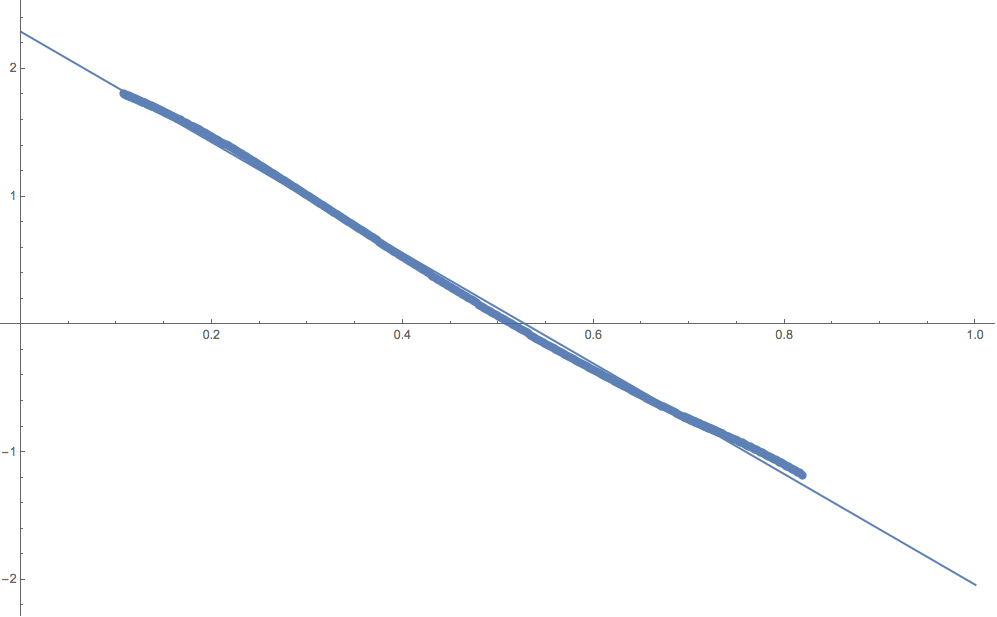
\includegraphics{assets/solar-electron-dist}
\caption{Solar electron density from Bahcall. 
Horizontal axis is the distance from the core of the sun normalized by the radius of the sun while the vertical axis is the number density of electrons in $\log_{10}(n/N_A)$.
The best fit for the line is 
$$ 2.3-4.3 \hat x .$$
So the equation of the number density distribution is
$$n = N_A 10^{2.3 - 4.3\hat x } .$$ }
\label{fig:solar-electron-dist}
\end{marginfigure}

The model using just exponential is not accurate however it is enough to make the point in MSW resonance.

So I choose a solar model in which the core density is $n(0) = 10^{-13}\mathrm{GeV}^{3}$. The distribution is \begin{equation*}
n =  10^{-13 - 4.3\hat x} \mathrm{GeV}^{3}.
\end{equation*}


The numerical results can be obtains by plugging this result into the differential equation solver. The result is shown in figure \ref{fig:numMSW-model-1}.



\begin{figure}
\centering
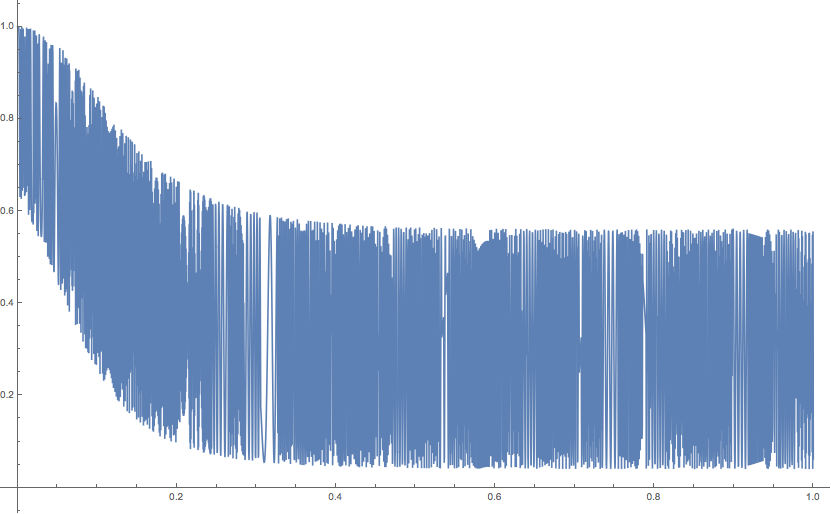
\includegraphics{assets/numMSW-model-1}
\caption{Numerical results for electron flavor neutrino when the electron density profile is $10^{-14 - 4.3\hat x} \mathrm{GeV}^{3}$.}
\label{fig:numMSW-model-1}
\end{figure}

\begin{figure}
\centering
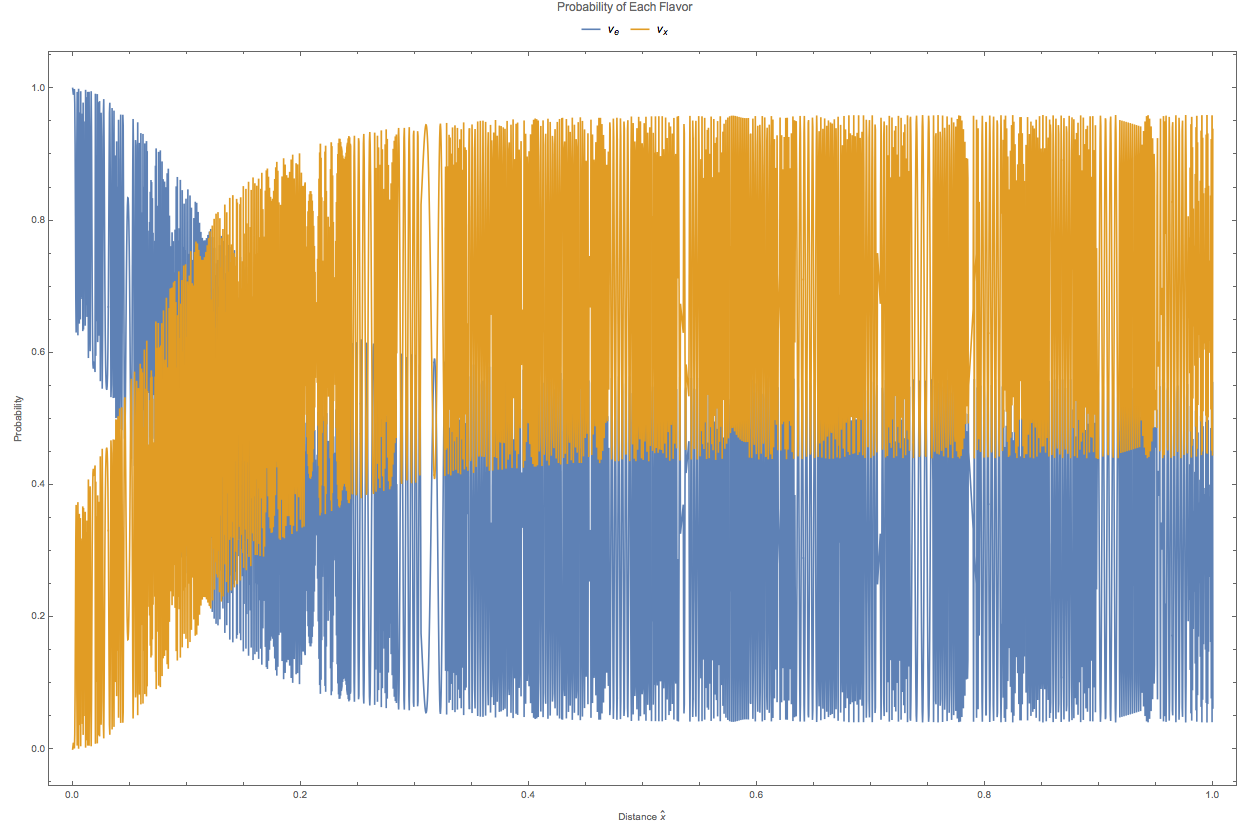
\includegraphics{assets/numericalMSW-model-3}
\caption{Numerical results for electron flavor neutrino probability and the other flavor neutrino probability when the electron density profile is $10^{-14 - 4.3\hat x} \mathrm{GeV}^{3}$.}
\label{fig:numMSW-model-3}
\end{figure}



\begin{figure}
\centering
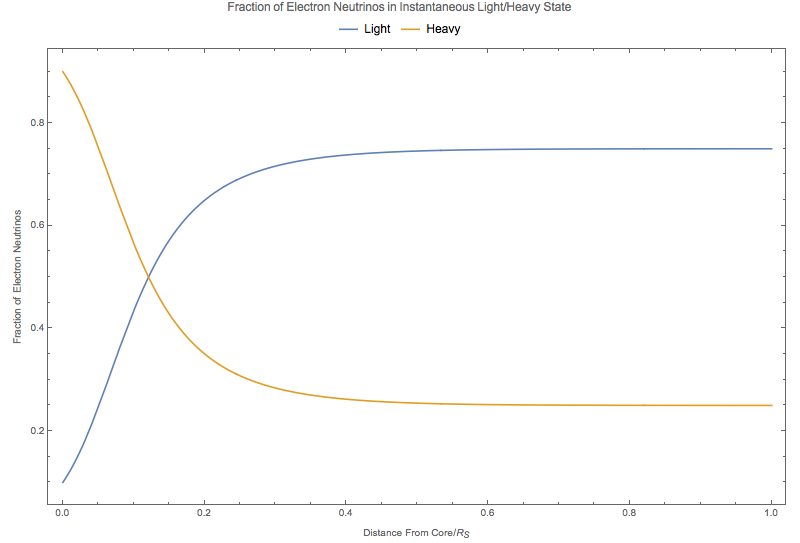
\includegraphics{assets/numericalMSW-model-lh.png}
\caption{The fraction of electron flavor in a $\ket{\nu_L}$ or $\ket{\nu_H}$ state as the neutrino passing through the sun from the core. This clearly shows a conversion of neutrino flavor.}
\label{fig:numericalMSW-model-lh}
\end{figure}



\begin{figure}
\centering
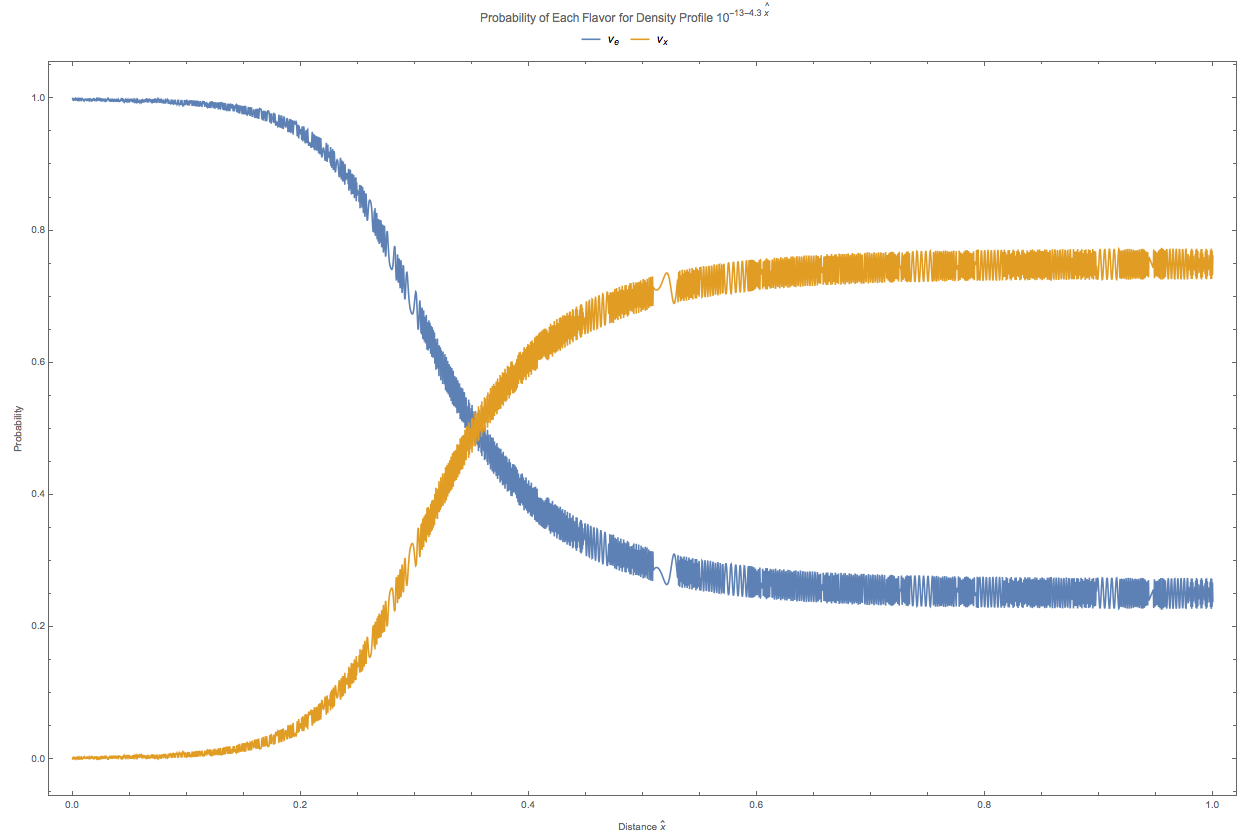
\includegraphics{assets/numericalMSW-model-2flavor-minus13-1}
\caption{Number density profile $n(\hat x) =  10^{-13 - 4.3\hat x}\mathrm{GeV^{3}}$.}
\label{fig:numericalMSW-model-2flavor-minus13-1}
\end{figure}







\subsection{Working in Vacuum Mass Eigenstates}

The third method is to work in vacuum mass eigenstates.

Vacuum part of the Hamiltonian is

\begin{align*}
\mathbf{H_{mvv}} = \frac{1}{2E} \begin{pmatrix}
m_1^2 & 0 & 0 \\
0 & m_2^2 & 0 \\
0 & 0 & m_3^2
\end{pmatrix}
\end{align*}

The matter interaction in flavor basis is

\begin{align*}
\mathbf{V_{mf}} = \sqrt{2}G_F n \mathrm{diag}{1,0,0}.
\end{align*}

Thus to work in vacuum mass eigenstates, we need a transformation

\begin{align*}
\mathbf{V_{mv}} = \mathbf{U^{-1}}\mathbf{V_{mf}} \mathbf{U}.
\end{align*}

Then the Hamiltonian becomes

\begin{equation*}
\mathbf{H_{m}} = \begin{pmatrix}
\frac{m_1^2}{2E} + \Delta U_{e1}^2 & \Delta U_{e1} U_{e2} & \Delta U_{e1} U_{e3} \\
\Delta U_{e2} U_{e1} & \frac{m_2^2}{2E} + \Delta U_{e2}^2 & \Delta U_{e2} U_{e3} \\
\Delta U_{e3} U_{e1} & \Delta U_{e3} U_{e2} & \frac{m_3^2}{2E} + \Delta U_{e3}^2
\end{pmatrix}
\end{equation*}

Trace of this Hamiltonian is $\mathrm{Tr}(\mathbf{H_m}) = \frac{m_1^2+m_2^2+m_3^2}{2E}+\Delta$. To find the traceless part, we can use the relation\ref{ohlsson2000}\footnote{arXiv:hep-ph/9910546}

\begin{equation*}
M = M_{traceless}+ \frac{1}{N} \mathrm{Tr}(M) I,
\end{equation*}

where $N$ is the rank.


The traceless part of Hamiltonian becomes

\begin{equation*}
\mathbf{H_{m}} = \begin{pmatrix}
\Delta U_{e1}^2 - \frac{1}{3}\Delta + \frac{1}{3}(\frac{m_1^2-m_2^2 + m_1^2-m_3^2}{2E}) & \Delta U_{e1}U_{e2} & \Delta U_{e1} U_{e3} \\
\Delta U_{e2} U_{e1} & \Delta U_{e2}^2 -\frac{1}{3}\Delta + \frac{1}{3}\frac{m_2^2 - m_1^2+m_2^2-m_3^2}{2E} & \Delta U_{e2}U_{e3} \\
\Delta U_{e1} U_{e3} & \Delta U_{e2} U_{e3} & \Delta U_{e3}^2 -\frac{1}{3} \Delta + \frac{1}{3} \frac{m_3^2 - m_1^2 + m_3^2-m_2^2 }{2E}
\end{pmatrix}
\end{equation*}

Define the following quantities\footnote{However only two of them are linearly independent.}

\begin{align*}
\Delta m_{12}^2 & = m_2^2 - m_1^2 \\
\Delta m_{23}^2 & = m_3^2 - m_2^2 \\
\Delta m_{13}^2 & = m_3^2 - m_1^2.
\end{align*}


We define an energy scale related to the radius of the sun

\begin{equation*}
\epsilon_S = \frac{1}{R_S}.
\end{equation*}

The EoM can be written in a dimensionless manner,

\begin{align*}
i\partial_{\hat x} \Psi_{m} =  \begin{pmatrix}
\hat\Delta U_{e1}^2 - \frac{1}{3}\hat\Delta + \frac{1}{3}(\frac{\Delta m_{12}^2 + \Delta m_{13}^2}{2E\epsilon_S}) & \hat\Delta U_{e1}U_{e2} & \hat\Delta U_{e1} U_{e3} \\
\hat\Delta U_{e2} U_{e1} & \hat\Delta U_{e2}^2 -\frac{1}{3}\hat\Delta + \frac{1}{3}\frac{\Delta m_{12}^2 + \Delta m_{23}^2}{2E\epsilon_S} & \hat\Delta U_{e2}U_{e3} \\
\hat\Delta U_{e1} U_{e3} & \hat\Delta U_{e2} U_{e3} & \hat\Delta U_{e3}^2 -\frac{1}{3} \hat\Delta + \frac{1}{3} \frac{\Delta m_{13}^2 + \Delta m_{23}^2 }{2E\epsilon_S} 
\end{pmatrix},
\end{align*}

where $\hat\Delta = \Delta/\epsilon_S$.


\subsection{Numerical Results of 3 Flavor}


The parameters for this calculation in units of $GeV^{whatever}$ are

\begin{align*}
numDen2(x) &= 10^{-12 - 4.3 x} \\
epSun &= 10^{-24}\\
deltaH(x) &= \sqrt[2] G_F numDen2(x)/epSun\\
deltam12sq &= 7.6\times 10^{-5}\times 10^{-18}\\
deltam13sq &= 2.3\times 10^{-3}\times 10^{-18}\\
deltam23sq &= deltam13sq - deltam12sq\\
ene &= 10^{-3}
\end{align*}

For these parameters there is only resonance for $\Delta m_{13}^2+\Delta m_{23}^2$.

A quick check over the different energy scales.

\begin{itemize}
\item Vacuum energy scales in normal hierarchy
\begin{align*}
\omega_{12}&= \frac{\Delta m_{12}^2}{2E} = 3.8\times 10^{-20}\mathrm{GeV}\\
\omega_{13}&= \frac{\Delta m_{13}^2}{2E} = 1.7\times 10^{-18}\mathrm{GeV}\\
\omega_{23}&= \frac{\Delta m_{23}^2}{2E} \approx \omega_{13}
\end{align*}
\item Matter related scale for density profile $10^{-14-4.3\hat x}$
\begin{equation*}
\Delta_1 = 1.6\times 10^{-19-4.3\hat x}\in [1.6\times 10^{-23.3},1.6\times 10^{-19}]
\end{equation*}

\item Matter related scale for density profile $10^{-13-4.3\hat x}$
\begin{equation*}
\Delta_1 = 1.6\times 10^{-18-4.3\hat x}\in [1.6\times 10^{-22.3},1.6\times 10^{-18}]
\end{equation*}



\end{itemize}



\begin{figure}
\centering
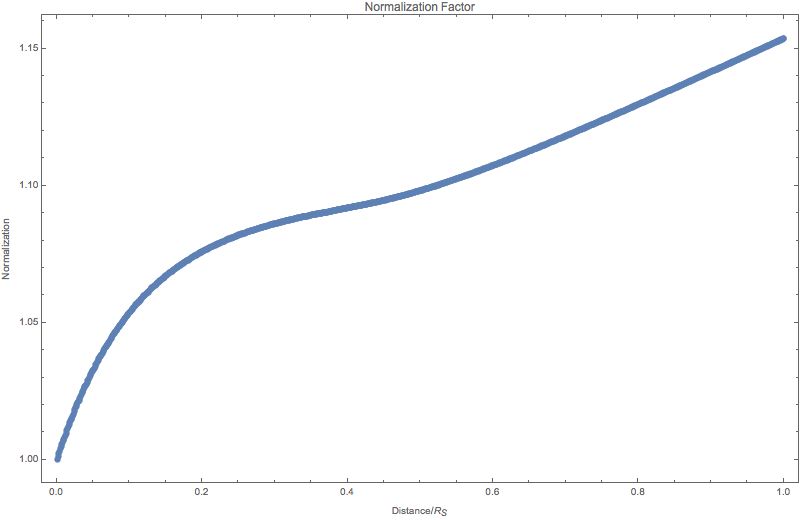
\includegraphics{assets/numericalMSW3Flavor-normalization}
\caption{Normalization factor as a function of distance.}
\label{fig:numericalMSW3Flavor-normalization}
\end{figure}


\begin{figure}
\centering
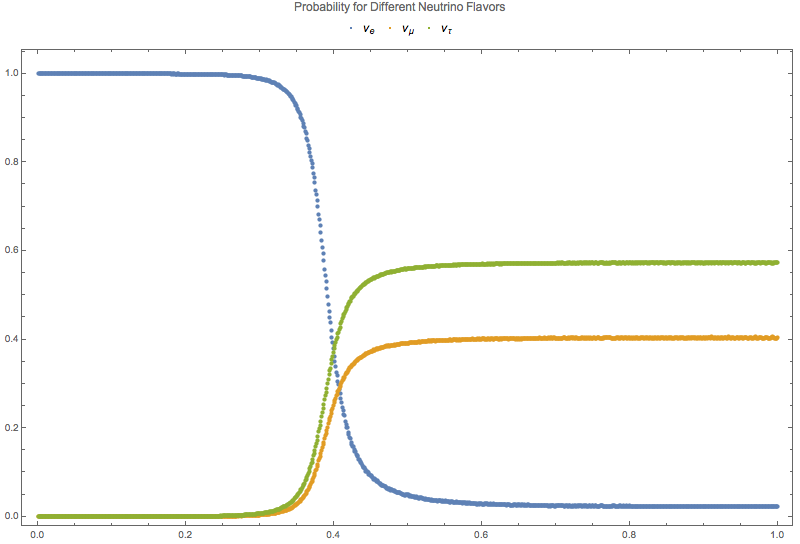
\includegraphics{assets/numericalMSW3Flavor-probabilities.png}
\caption{Probability for each flavor of neutrinos.}
\label{fig:numericalMSW3Flavor-probabilities}
\end{figure}



Applying a number density function $numDen2(x) = 10^{-13 - 4.3 x}$ to the system, the small scale oscillations are revived,

\begin{figure}
\centering
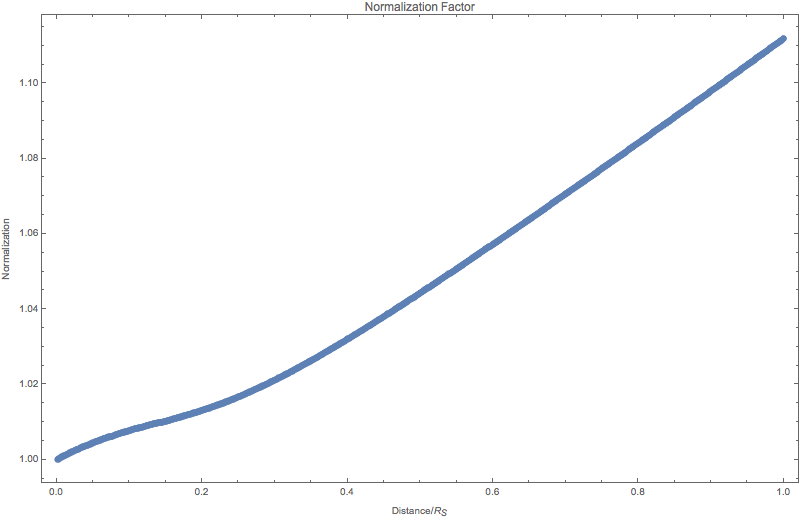
\includegraphics{assets/numericalMSW3Flavor-2-norm}
\caption{Normalization of the states for numerical 3 flavor oscillation in the sun with density profile $10^{-13 - 4.3 x}$.}
\label{fig:numericalMSW3Flavor-2-norm}
\end{figure}


\begin{figure}
\centering
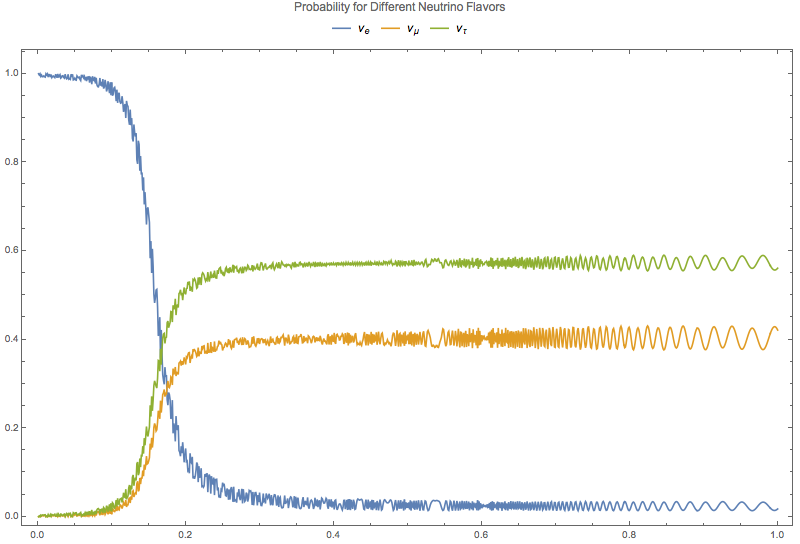
\includegraphics{assets/numericalMSW3Flavor-2-probability}
\caption{Numerical results for 3 flavor oscillation in the sun with density profile $10^{-13 - 4.3 x}$.}
\label{fig:numericalMSW3Flavor-2-probability}
\end{figure}


\begin{marginfigure}[6\baselineskip]
\centering
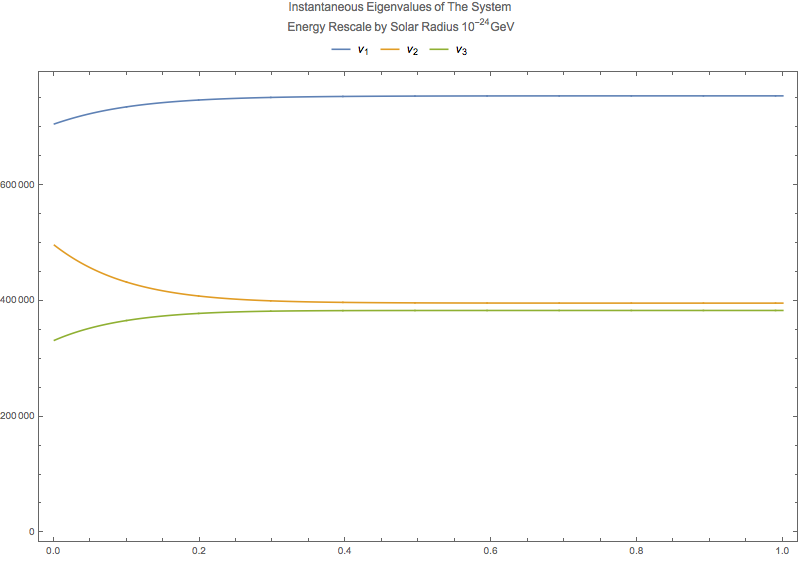
\includegraphics{assets/numericalMSW3Flavor-minus14-Inst-Eigen-Energies.png}
\caption{Eigenenergies for density profile $10^{-13 - 4.3 x}$.}
\label{fig:numericalMSW3Flavor-minus14-Inst-Eigen-Energies}
\end{marginfigure}


\begin{figure}
\centering
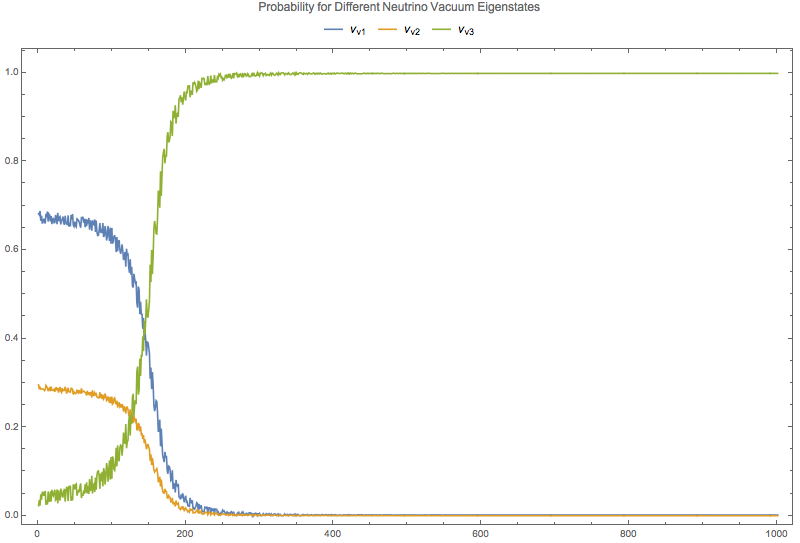
\includegraphics{assets/numericalMSW3Flavor-vac-eigen-prob.png}
\caption{Survival probabilities for different vacuum mass eigenstates for 3 flavor oscillation in the sun with density profile $10^{-13 - 4.3 x}$.}
\label{fig:my_label}
\end{figure}


\begin{marginfigure}[2\baselineskip]
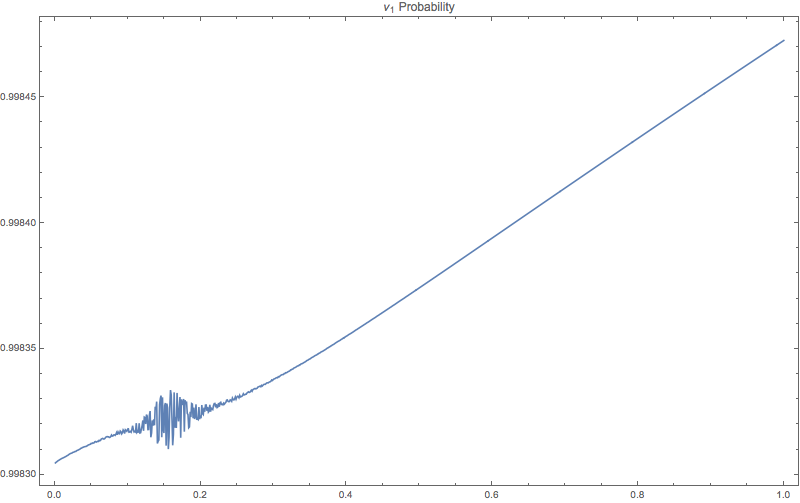
\includegraphics{assets/numericalMSW3Flavor-Inst-Eigen-prob-1.png}
\caption{Probability for the first instantaneous eigenstate for matter profile $10^{-13 - 4.3 x}$.}
\label{fig:numericalMSW3Flavor-Inst-Eigen-prob-1}
\end{marginfigure}


\begin{marginfigure}[2\baselineskip]
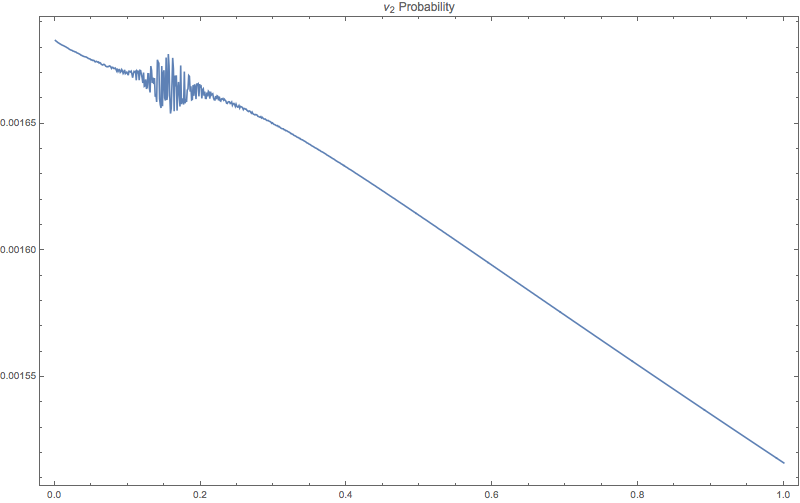
\includegraphics{assets/numericalMSW3Flavor-Inst-Eigen-prob-2.png}
\caption{Probability for the second instantaneous eigenstate for matter profile $10^{-13 - 4.3 x}$.}
\label{fig:numericalMSW3Flavor-Inst-Eigen-prob-2}
\end{marginfigure}

\begin{marginfigure}[2\baselineskip]
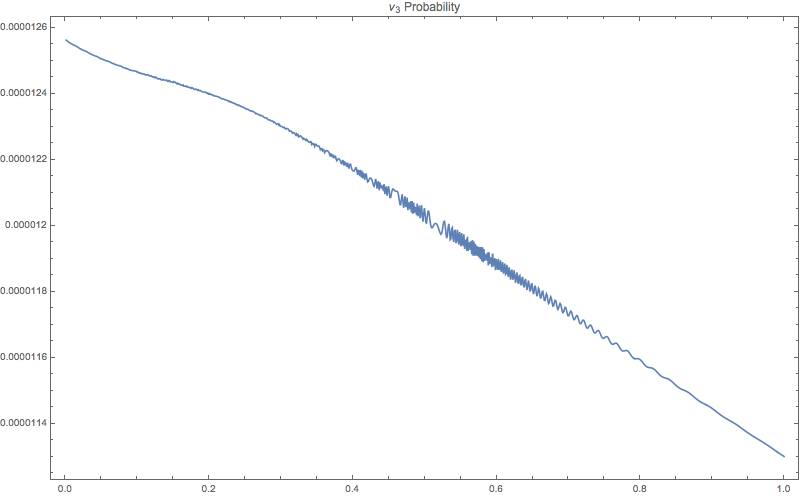
\includegraphics{assets/numericalMSW3Flavor-Inst-Eigen-prob-3.png}
\caption{Probability for the third instantaneous eigenstate for matter profile $10^{-13 - 4.3 x}$.}
\label{fig:numericalMSW3Flavor-Inst-Eigen-prob-3}
\end{marginfigure}



\begin{figure}
\centering
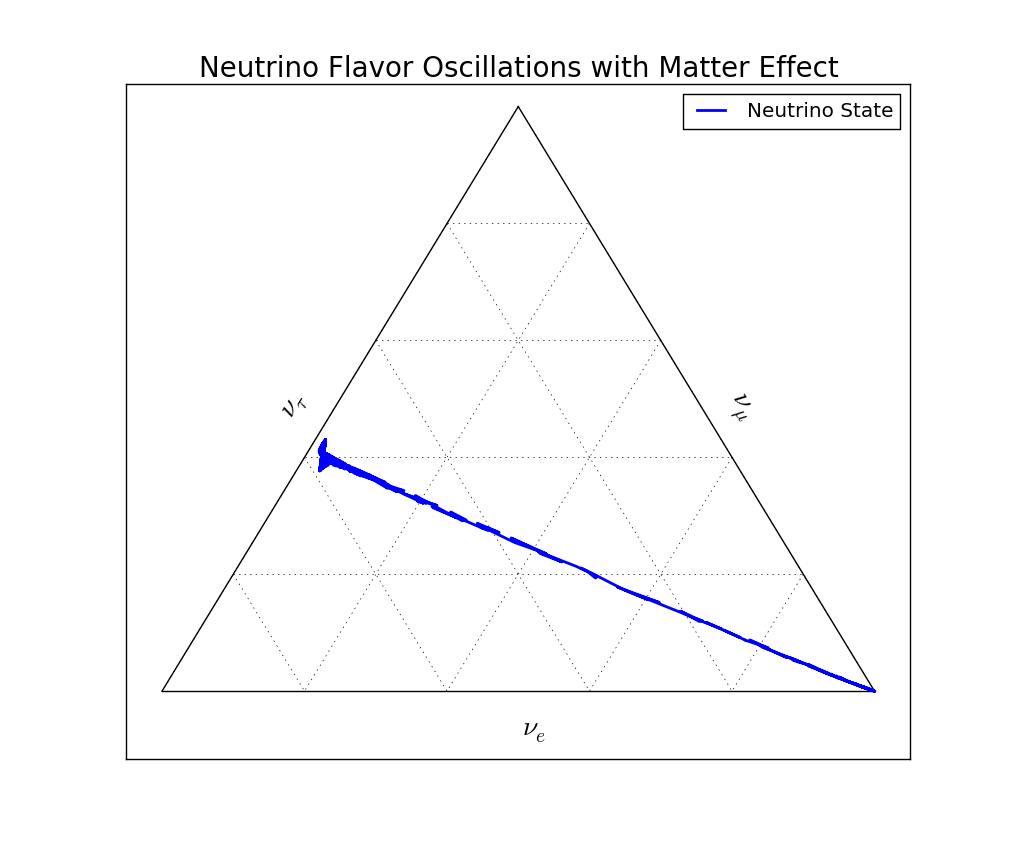
\includegraphics{assets/ternary/mass-1}
\caption{Ternary diagram for MSW effect.}
\label{fig:ternary-mass-1}
\end{figure}

\begin{figure}
\centering
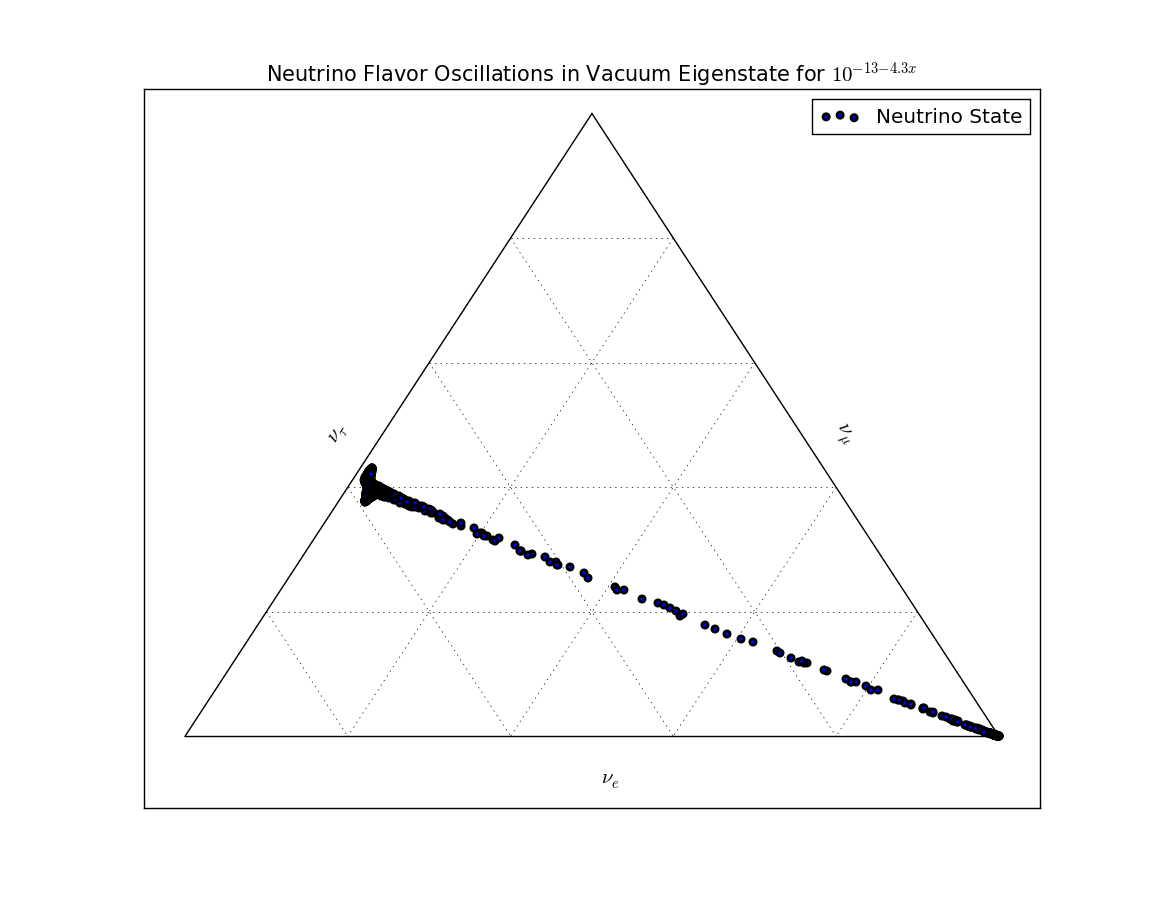
\includegraphics{assets/ternary/mass-1-scatter.png}
\caption{Ternary diagram for MSW effect.}
\label{fig:ternary-mass-1-scatter}
\end{figure}



\begin{figure}
\centering
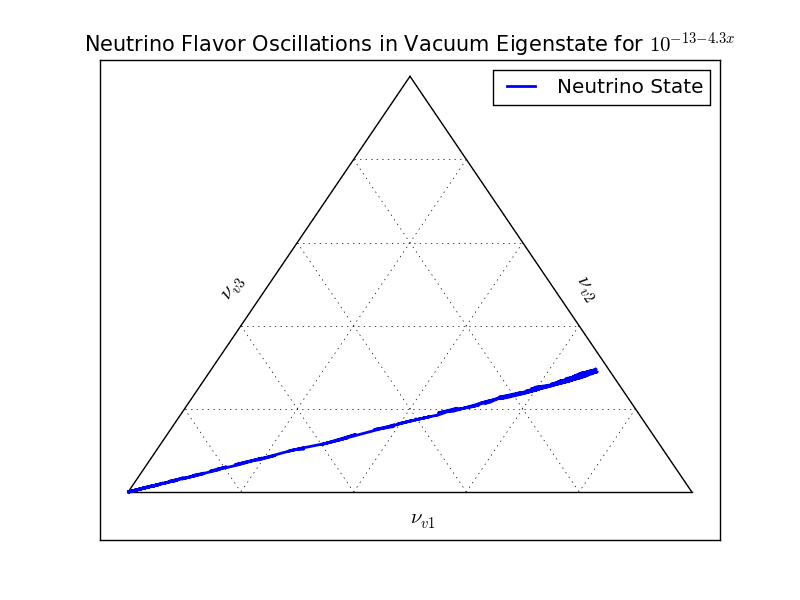
\includegraphics{assets/ternary/matter-vac-eigen-e-1.png}
\caption{Ternary diagram for vacuum eigenstates}
\label{fig:matter-vac-eigen-e-1}
\end{figure}



\begin{figure}
\centering
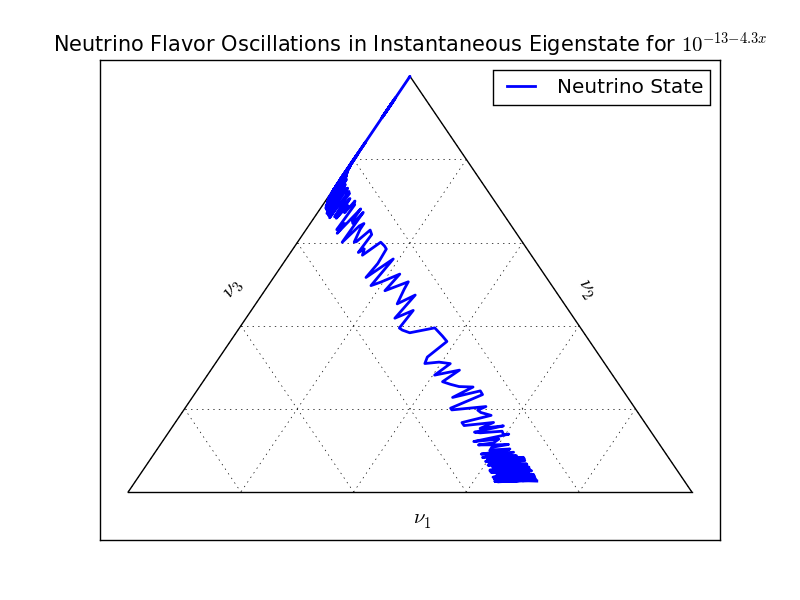
\includegraphics{assets/ternary/matter-inst-eigen-e-1.png}
\caption{Ternary diagram for instantaneous eigenstates}
\label{fig:matter-inst-eigen-e-1}
\end{figure}



\begin{figure}
\centering
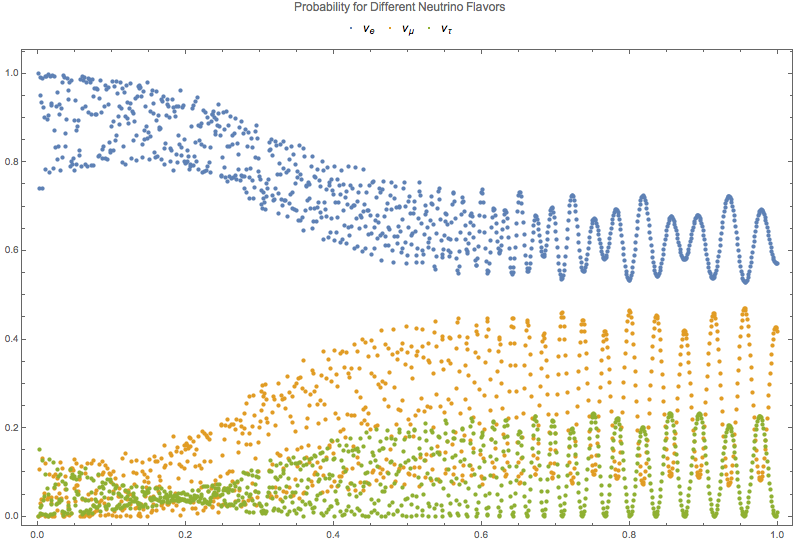
\includegraphics{assets/numericalMSW3Flavor-minus14matter.png}
\caption{Numerical results for 3 flavor oscillation in the sun with density profile $10^{-14 - 4.3 x}$.}
\label{fig:numericalMSW3Flavor-minus14matter}
\end{figure}



\begin{figure}
\centering
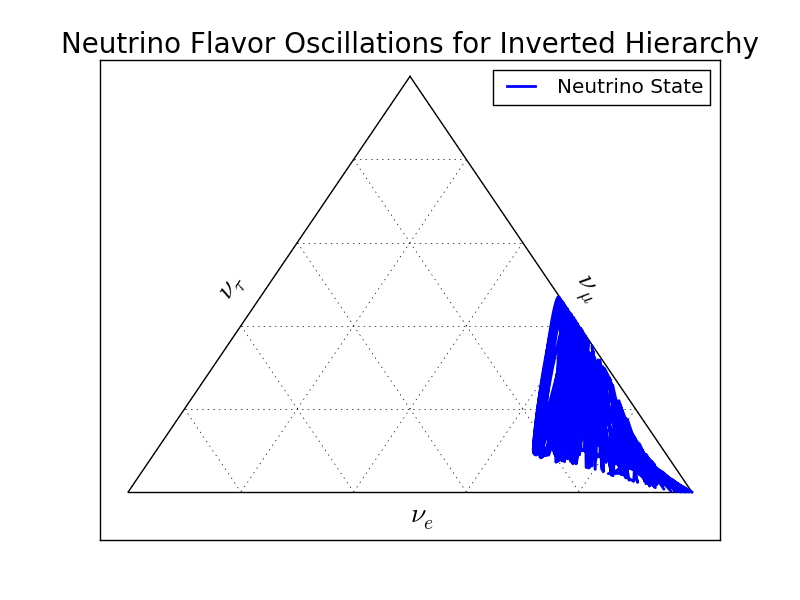
\includegraphics{assets/ternary/matter-minus14-1.png}
\caption{Ternary diagram for MSW effect with matter density profile $10^{-14 - 4.3 x}$.}
\label{fig:ternary-mass-1}
\end{figure}







\section{Ternary Diagrams}



\begin{figure}
\centering
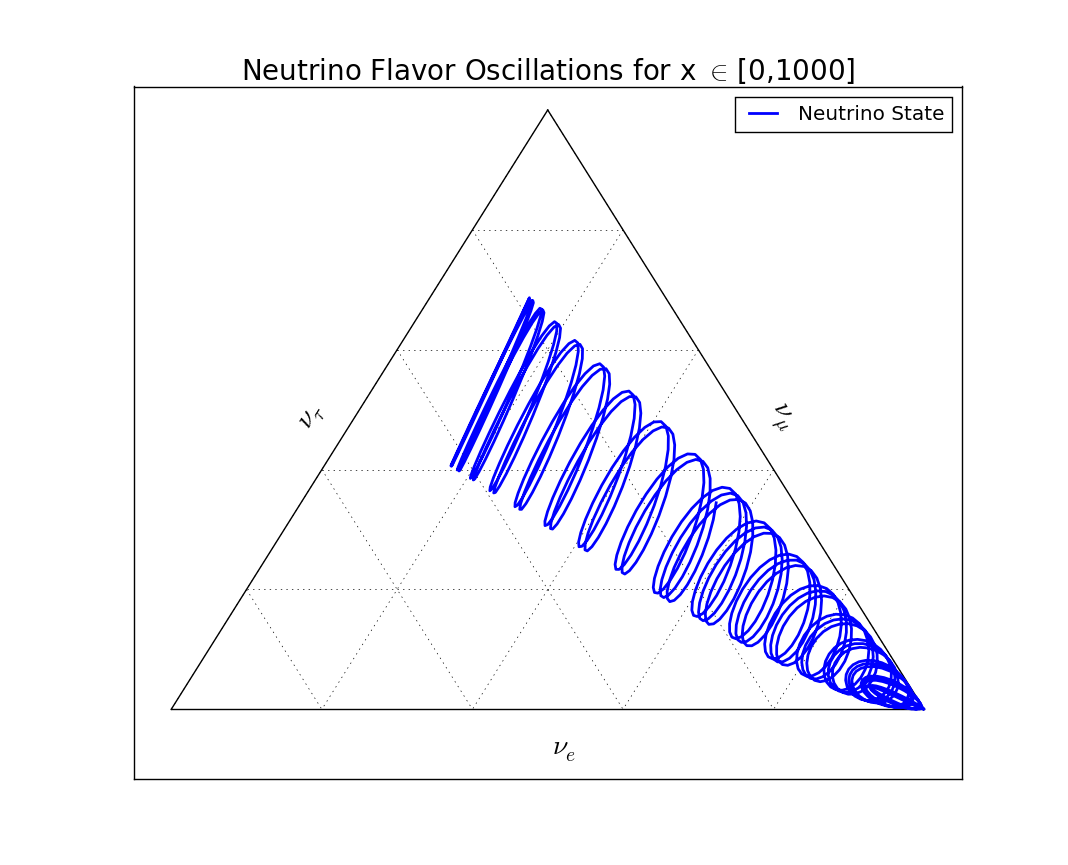
\includegraphics{assets/ternary/1000-1}
\caption{ 
theta12 = 33.36/180*Pi;\newline
theta13 = 8.66/180*Pi;\newline
theta23 = 40/180*Pi;\newline
deltacp = 0;\newline
m1sq = 0.01;\newline
m2sq = m1sq + 0.000079;\newline
oneFourE = 100; 
}
\end{figure}



\begin{figure}
\centering
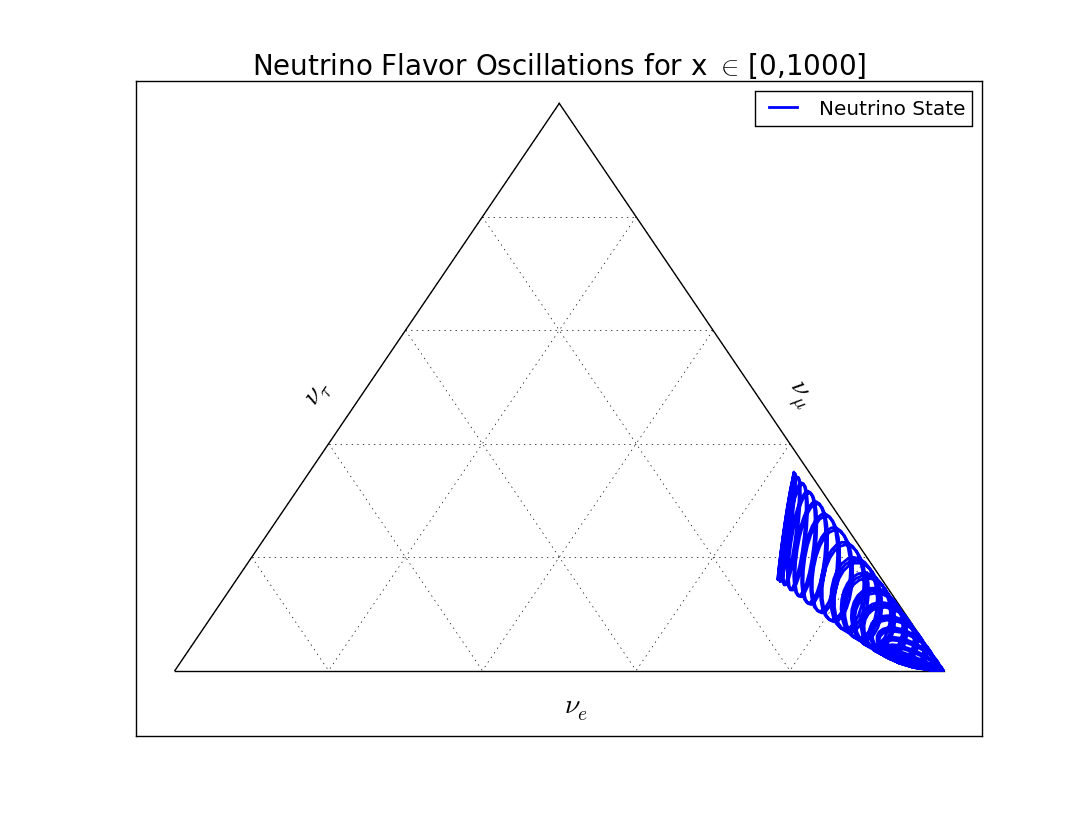
\includegraphics{assets/ternary/1000-2}
\caption{ Reduce theta12 to half of the original value \newline
theta12 = 33.36/180*Pi*1/2;\newline
theta13 = 8.66/180*Pi;\newline
theta23 = 40/180*Pi;\newline
deltacp = 0;\newline
m1sq = 0.01;\newline
m2sq = m1sq + 0.000079;\newline
oneFourE = 100; 
}
\end{figure}


\begin{figure}
\centering
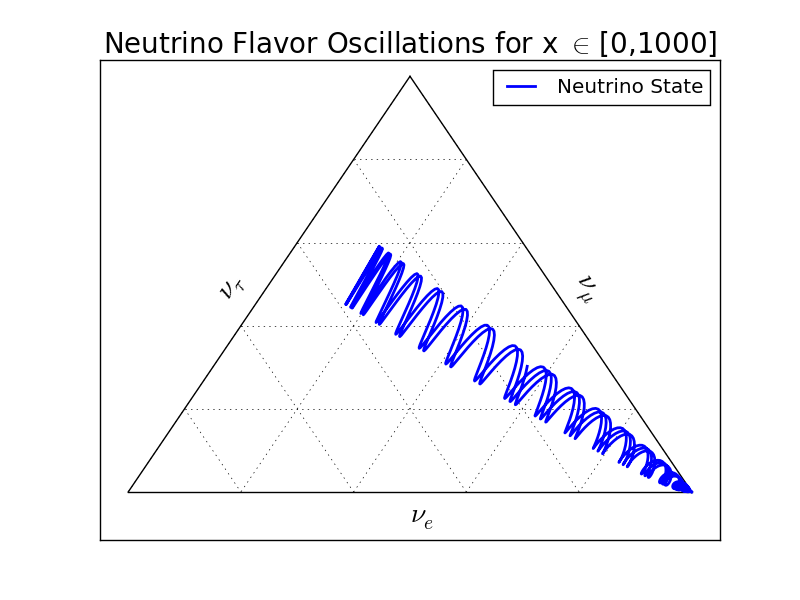
\includegraphics{assets/ternary/1000-3}
\caption{ Reduce theta13\newline
theta12 = 33.36/180*Pi;\newline
theta13 = 8.66/180*Pi*1/2;\newline
theta23 = 40/180*Pi;\newline
deltacp = 0;\newline
m1sq = 0.01;\newline
m2sq = m1sq + 0.000079;\newline
oneFourE = 100; 
}
\end{figure}




\begin{figure}
\centering
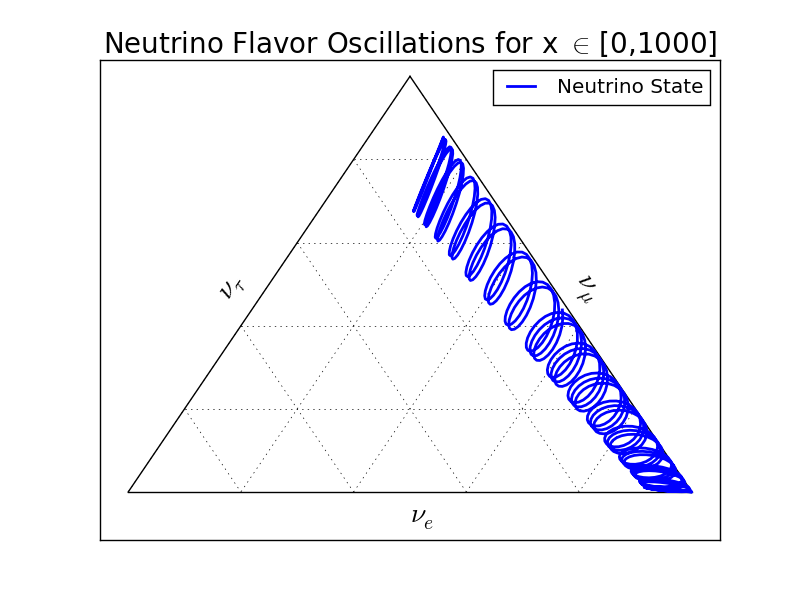
\includegraphics{assets/ternary/1000-4}
\caption{ Reduce theta23 \newline
theta12 = 33.36/180*Pi;\newline
theta13 = 8.66/180*Pi;\newline
theta23 = 40/180*Pi*1/2;\newline
deltacp = 0;\newline
m1sq = 0.01;\newline
m2sq = m1sq + 0.000079;\newline
oneFourE = 100; 
}
\end{figure}



\begin{figure}
\centering
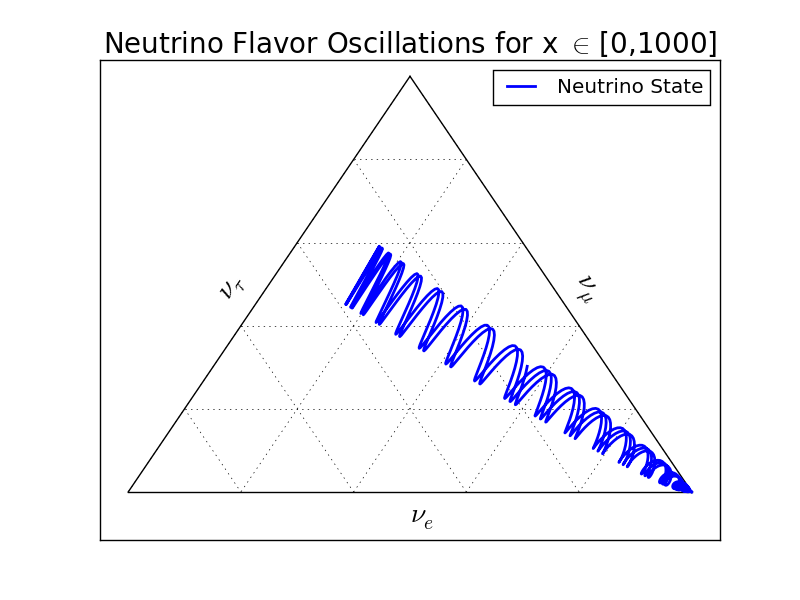
\includegraphics{assets/ternary/1000-3}
\caption{ Increase $deltam2^2-deltam1^2$\newline
theta12 = 33.36/180*Pi;\newline
theta13 = 8.66/180*Pi;\newline
theta23 = 40/180*Pi;\newline
deltacp = 0;\newline
m1sq = 0.01;\newline
m2sq = m1sq + 0.000079*10;\newline
oneFourE = 100; 
}
\end{figure}




\begin{figure}
\centering
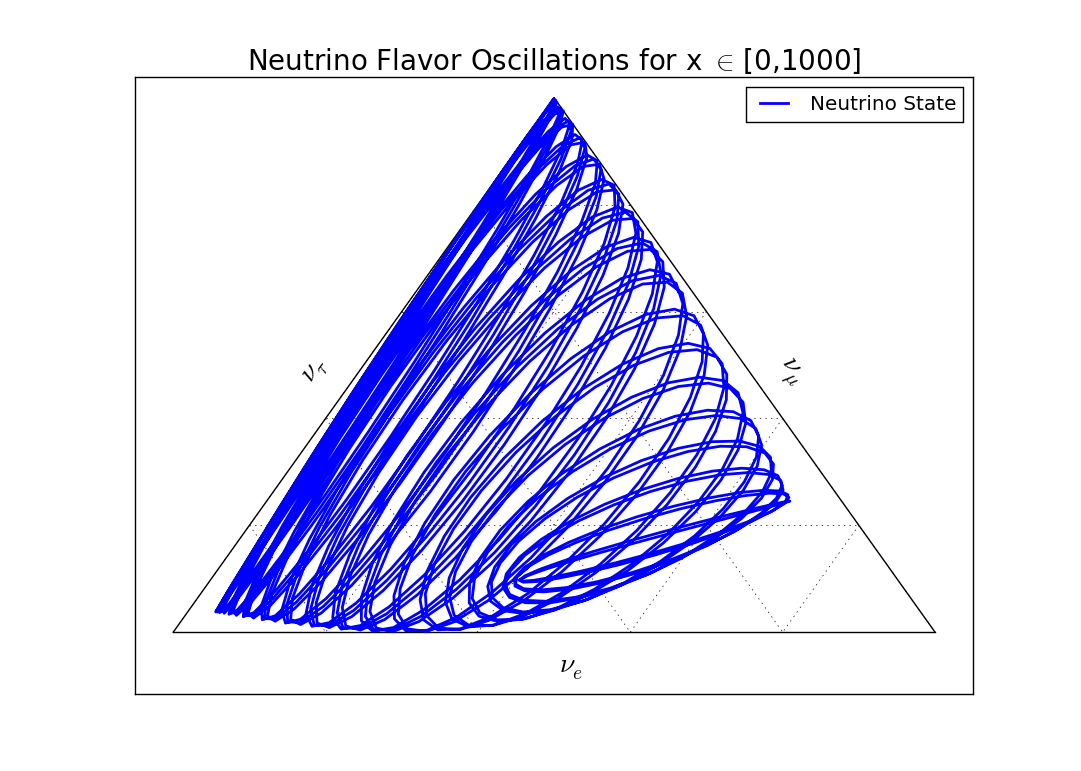
\includegraphics{assets/ternary/1000-mu-1}
\caption{ Starting from all $\nu_\mu$ \newline
theta12 = 33.36/180*Pi;\newline
theta13 = 8.66/180*Pi;\newline
theta23 = 40/180*Pi;\newline
deltacp = 0;\newline
m1sq = 0.01;\newline
m2sq = m1sq + 0.000079;\newline
oneFourE = 100; 
}
\end{figure}
























%% As we said before, % I forgot what was that.

\subsection{Decapitated - Solar Density Profile}



The solar density profile can be determined using simple gravitational theory and nuclear physics models.

The mass contained in a spherical shell $dr$ is

\begin{equation}
    dm = 4\pi r^2 \rho dr ,
\end{equation}

which is assuming spherical symmetry.

The gravitational potential for each unit of mass can generate force as gravitational attraction, which is

\begin{equation*}
    \frac{dv}{dr} = \frac{G m}{r^2}.
\end{equation*}

The balance between pressure and gravity shows that

\begin{equation*}
    \frac{dv}{dr} \rho + \frac{dp}{dr} = 0.
\end{equation*}

The result of these relations is a rather intuitive relation between density and pressure, which is not solvable until we find another relation between them.

\begin{equation*}
    \frac{1}{r^2} \frac{d}{dr} \left( \frac{r^2}{\rho} \frac{dp}{dr} \right) = -4\pi G\rho.
\end{equation*}

To be simple, we will use Eddington model to solve the density profile, which gives us the relation

\begin{equation*}
    p = K \rho^{4/3},
\end{equation*}


where 
\begin{equation*}
    K = \left(  \left( \frac{k}{m_p} \frac{3}{\alpha} \frac{\beta}{\mu^4(1-\beta)^4}  \right)^4  \right)^{1/3}.
\end{equation*}




\bibliography{ref}
\bibliographystyle{plainnat}


\end{document}
